%Version 2.1 April 2023
% See section 11 of the User Manual for version history
%
%%%%%%%%%%%%%%%%%%%%%%%%%%%%%%%%%%%%%%%%%%%%%%%%%%%%%%%%%%%%%%%%%%%%%%
%%                                                                 %%
%% Please do not use \input{...} to include other tex files.       %%
%% Submit your LaTeX manuscript as one .tex document.              %%
%%                                                                 %%
%% All additional figures and files should be attached             %%
%% separately and not embedded in the \TeX\ document itself.       %%
%%                                                                 %%
%%%%%%%%%%%%%%%%%%%%%%%%%%%%%%%%%%%%%%%%%%%%%%%%%%%%%%%%%%%%%%%%%%%%%

\documentclass[sn-basic,referee,lineno,pdflatex]{sn-jnl}

%%%% Standard Packages
%%<additional latex packages if required can be included here>

\usepackage{graphicx}%
\usepackage{multirow}%
\usepackage{amsmath,amssymb,amsfonts}%
\usepackage{amsthm}%
\usepackage{mathrsfs}%
\usepackage[title]{appendix}%
\usepackage{xcolor}%
\usepackage{textcomp}%
\usepackage{manyfoot}%
\usepackage{booktabs}%
\usepackage{algorithm}%
\usepackage{algorithmicx}%
\usepackage{algpseudocode}%
\usepackage{listings}%
%%%%

%%%%%=============================================================================%%%%
%%%%  Remarks: This template is provided to aid authors with the preparation
%%%%  of original research articles intended for submission to journals published
%%%%  by Springer Nature. The guidance has been prepared in partnership with
%%%%  production teams to conform to Springer Nature technical requirements.
%%%%  Editorial and presentation requirements differ among journal portfolios and
%%%%  research disciplines. You may find sections in this template are irrelevant
%%%%  to your work and are empowered to omit any such section if allowed by the
%%%%  journal you intend to submit to. The submission guidelines and policies
%%%%  of the journal take precedence. A detailed User Manual is available in the
%%%%  template package for technical guidance.
%%%%%=============================================================================%%%%

\usepackage{booktabs}
\usepackage{longtable}
\usepackage{array}
\usepackage{multirow}
\usepackage{wrapfig}
\usepackage{float}
\usepackage{colortbl}
\usepackage{pdflscape}
\usepackage{tabu}
\usepackage{threeparttable}
\usepackage{threeparttablex}
\usepackage[normalem]{ulem}
\usepackage{makecell}
\usepackage{xcolor}
\usepackage{siunitx}

  \newcolumntype{d}{S[
    input-open-uncertainty=,
    input-close-uncertainty=,
    parse-numbers = false,
    table-align-text-pre=false,
    table-align-text-post=false
  ]}
  


\raggedbottom




% tightlist command for lists without linebreak
\providecommand{\tightlist}{%
  \setlength{\itemsep}{0pt}\setlength{\parskip}{0pt}}





\begin{document}


\title[Watershed nutrient loading and water quality in a subtropical
estuary]{Assessing linkages between watershed nutrient loading and water
quality in a subtropical estuary with semiparametric models.}

%%=============================================================%%
%% Prefix	-> \pfx{Dr}
%% GivenName	-> \fnm{Joergen W.}
%% Particle	-> \spfx{van der} -> surname prefix
%% FamilyName	-> \sur{Ploeg}
%% Suffix	-> \sfx{IV}
%% NatureName	-> \tanm{Poet Laureate} -> Title after name
%% Degrees	-> \dgr{MSc, PhD}
%% \author*[1,2]{\pfx{Dr} \fnm{Joergen W.} \spfx{van der} \sur{Ploeg} \sfx{IV} \tanm{Poet Laureate}
%%                 \dgr{MSc, PhD}}\email{iauthor@gmail.com}
%%=============================================================%%

\author*[1]{\fnm{Michael} \sur{Schramm} }\email{\href{mailto:michael.schramm@ag.tamu.edu}{\nolinkurl{michael.schramm@ag.tamu.edu}}}



  \affil*[1]{\orgdiv{Texas Water Resources Institute}, \orgname{Texas
A\&M AgriLife Research}, \orgaddress{\city{College
Station}, \country{United
States}, \postcode{77840}, \state{TX}, \street{1001 Holleman Dr.~E.}}}

\abstract{Lavaca Bay is a small secondary embayment on the Texas coast
that is displaying early signals of water quality degradation. This
study applied a semiparametric approach to assess both watershed
nutrient loads and the responses in estuary water quality to nutrient
loading and streamflow. Cross-validation indicated that, despite data
constraints, semiparametric models performed well at nutrient load
prediction. Based on these models, delivered annual nutrient loads
varied substantially from year to year. In contrast, minimal changes in
calculated flow-normalized loads indicate that changes in nutrient
loading were driven by natural variation in precipitation and runoff as
opposed to changes in nonpoint sources. Estuary water quality models did
not identify significant long-term changes within Lavaca Bay for
dissolved oxygen or chlorophyll-\emph{a}. However, site specific
long-term increases in both organic and inorganic nitrogen are
concerning. Further analysis found freshwater inflow was a strong driver
of nutrient and chlorophyll-\emph{a} concentrations within Lavaca Bay
but there was no evidence that changes in nutrient loading explained
variation in dissolved oxygen or chlorophyll-\emph{a} concentrations. In
addition to providing a baseline assessment of watershed nutrient
loading and water quality responses in the Lavaca Bay watershed, this
study provides methodological support for the use of semiparametric
methods in load regression models and estuary assessments.}

\keywords{key, dictionary, word}



\maketitle

\hypertarget{sec1}{%
\section{Introduction}\label{sec1}}

Like many coastal areas globally, the coastal watersheds along the Texas
Gulf coast are facing pressures from increasing population, increases in
point source and non-point source pollution and alterations to
freshwater flows that degrade water quality in downstream estuaries
\citep{bricker_effects_2008, kennicuttWaterQualityGulf2017, bugica_water_2020}.
Despite these escalating pressures, national scale assessments have
classified coastal estuaries in Texas as moderate or low risk for
eutrophic conditions \citep{bricker_effects_2008}. However, a suite of
recent studies indicates that estuary water quality dynamics in both
agriculturally dominated and urban watersheds within Texas are in fact
expressing conditions that are increasingly conducive to algal blooms
and eutrophication
\citep{wetzWaterQualityDynamics2016, wetz_exceptionally_2017, bugica_water_2020, chinPhytoplanktonBiomassCommunity2022}.
With identification of localized areas of estuary water quality concern
along the Texas coast \citep{bugica_water_2020}, localized studies are
being prioritized to better inform management actions.

This project aims to provide an assessment of nutrient loading and water
quality responses in Lavaca Bay, Texas. Lavaca Bay is a secondary bay in
the larger Matagorda Bay system located roughly halfway between Houston,
Texas and Corpus Christi, Texas. Lavaca Bay faces substantial challenges
associated with legacy contamination but general water quality
parameters such as dissolved oxygen (DO), nutrients, and biological
parameters have been well within state water quality standards. More
recently identified long-term declines in abundance, biomass, and
diversity of benthic fauna in Lavaca Bay have been linked to reductions
in freshwater inflows and changes in estuary salinity
\citep{beserespollackLongtermTrendsResponse2011, palmerImpactsDroughtsLow2015, montagnaAssessmentRelationshipFreshwater2020}
and are a concern to local stakeholders. Water quality assessments
identified monotonic increases in total phosphorus (TP), orthophosphate,
total Kjeldahl nitrogen (TKN), and chlorophyll-\emph{a} at sites within
Lavaca Bay \citep{bugica_water_2020}. Although long-term changes in DO
concentrations were not identified, the trends in nutrient
concentrations are concerning due to the role of nitrogen as a limiting
factor for primary production in many Texas estuaries
\citep{gardnerNitrogenFixationDissimilatory2006, houTransformationFateNitrate2012, doradoUnderstandingInteractionsFreshwater2015, paudelRelationshipSuspendedSolids2019, wetz_exceptionally_2017}
and the ramifications that changes in nitrogen loadings could have for
productivity and eutrophication in Lavaca Bay.

There are ongoing efforts between local, state, and federal agencies to
address water quality impairments in the freshwater portions of the
Lavaca Bay watershed
\citep{jainTechnicalSupportDocument2021, schrammLavacaRiverWatershed2018, bertholdDirectMailingEducation2021}.
However, at a statewide scale, these approaches have shown limited
success and emphasize a need for improved efforts at assessing and
linking management actions with downstream water quality to identify and
replicate effective management actions across the state
\citep{schrammTotalMaximumDaily2022}. The identification and
communication of changes and trends in water quality is complicated by
the fact that trends are often non-linear and confounded by
precipitation and runoff that hinder traditional analysis
\citep{wazniakLinkingWaterQuality2007, lloydMethodsDetectingChange2014}.
The development and application of statistical methods such as Weighted
Regressions on Time, Discharge and Season
\citep[WRTDS,][]{hirschWeightedRegressionsTime2010} and Generalized
Additive Models \citep[GAMs,][]{woodFastStableRestricted2011} has
provided effective tools for researchers to quantify and communicate
non-linear changes in river and estuary pollutant loadings.

WRTDS calculates a time series of in stream concentrations or loads
(daily, monthly, or annually) and flow-normalized estimates of
concentrations and loads using locally weighted regresssion for unique
combinations of time, discharge, and season. WRTDS has been widely used
to assess and identify trends in riverine nutrients
\citep{oelsner_recent_2019, stackpooleLongTermMississippi2021},
chlorides \citep{stetsIncreasingChlorideRivers2018}, and other
pollutants of concern \citep{shodaWaterqualityTrendsRivers2019}. WRTDS
has also been succesfully adapted to assess trends in estuarine water
quality concentrations \citep{beckFourDecadesWater2018}.

While WRTDS is a statistical approach developed specifically for water
quality applications, GAMs are a broadly applicable statistical method.
GAMs are a semiparametric extension of generalized linear models where
the linear predictor is represented as the sum of multiple unknown
smooth functions and parametric linear predictors
\citep{woodFastStableRestricted2011}. Although the underlying parameter
estimation procedure of GAMs is substantially different than WRTDS, both
the functional form and results have been demonstrated to be similar
\citep{beckNumericalQualitativeContrasts2017}. Water quality
applications of GAMs include river and catchment nutrient concentration
and load models
\citep{wangLoadEstimationUncertainties2011, kroonRiverLoadsSuspended2012, kuhnertQuantifyingTotalSuspended2012, robson_prediction_2015-1, hagemannEstimatingNutrientOrganic2016, mcdowell_implications_2021, biagi_novel_2022}.
GAMs can also be used to identify non-linear temporal trends (including
flow-normalized trends) in pollutant concentrations and loads
\citep{beckNumericalQualitativeContrasts2017, murphyGeneralizedAdditiveModel2019}.
Recently GAMs have also been used to link water quality responses in
receiving water bodies to changes in nutrient inputs
\citep{murphyNutrientImprovementsChesapeake2022}.
\citet{beckNumericalQualitativeContrasts2017} provides a substantial
discussion on the differences (and similarities) between GAMs and WRTDS
for water quality applications.

To provide actionable information for resource managers in Lavaca Bay,
water quality conditions must be evaluated relative to changes in
natural environmental drivers to better understand and manage potential
human impacts. This study utilizes GAMs to develop estimates of
delivered and flow-normalized nutrient loads and assess changes in loads
delivered to Lavaca Bay. GAMs were chosen over other regression-based
approached for use in this study due to; (1) the ability to easily
explore and incorporate different model terms; (2) the incorporation of
non-liner smooth functions that do not require explicit a priori
knowledge of the expected shape; and (3) inclusion of a link function
that related the expected value of the response to linear predictors
thus avoiding unneeded data transformations and bias corrections. The
study also assesses the response of water quality parameters in Lavaca
Bay over time and in response to freshwater inflow controlled for
seasonality and to watershed nutrient loads that are controlled for
environmentally driven variation.

\hypertarget{sec2}{%
\section{Methods}\label{sec2}}

\hypertarget{location-and-data}{%
\subsection{Location and Data}\label{location-and-data}}

Lavaca Bay is 190 km\textsuperscript{2} with the majority of freshwater
inflow provided by the Lavaca and Navidad River systems
(Figure~\ref{fig:fig1}). The Garcitas-Arenosa, Placedo Creek, and Cox
Bay watersheds provide additional freshwater inflows. The entire
watershed land area is 8,149 km\textsuperscript{2} and primarily rural.
Watershed land cover and land use is 50\% grazed pasture and rangeland,
20\% cultivated cropland (primarily rows crops such as corn, cotton, and
sorghum), and 5\% suburban/urban. Pasture and rangeland is concentrated
in the Lavaca River watershed, while cultivated crops are generally
located along the eastern tributaries of the Navidad river. The Lavaca
and Navidad River watersheds are a combined 5,966 km\textsuperscript{2},
or approximately 73\% of the entire Lavaca Bay watershed area. Discharge
from the Navidad River is regulated by Lake Texana which has been in
operation since 1980. Lake Texana provides 0.210 km\textsuperscript{3}
of water storage and discharges into the tidal section of the Navidad
River which ultimately joins the tidal section of the Lavaca River 15 km
upstream of the confluence with the Lavaca Bay.

\begin{figure}

{\centering 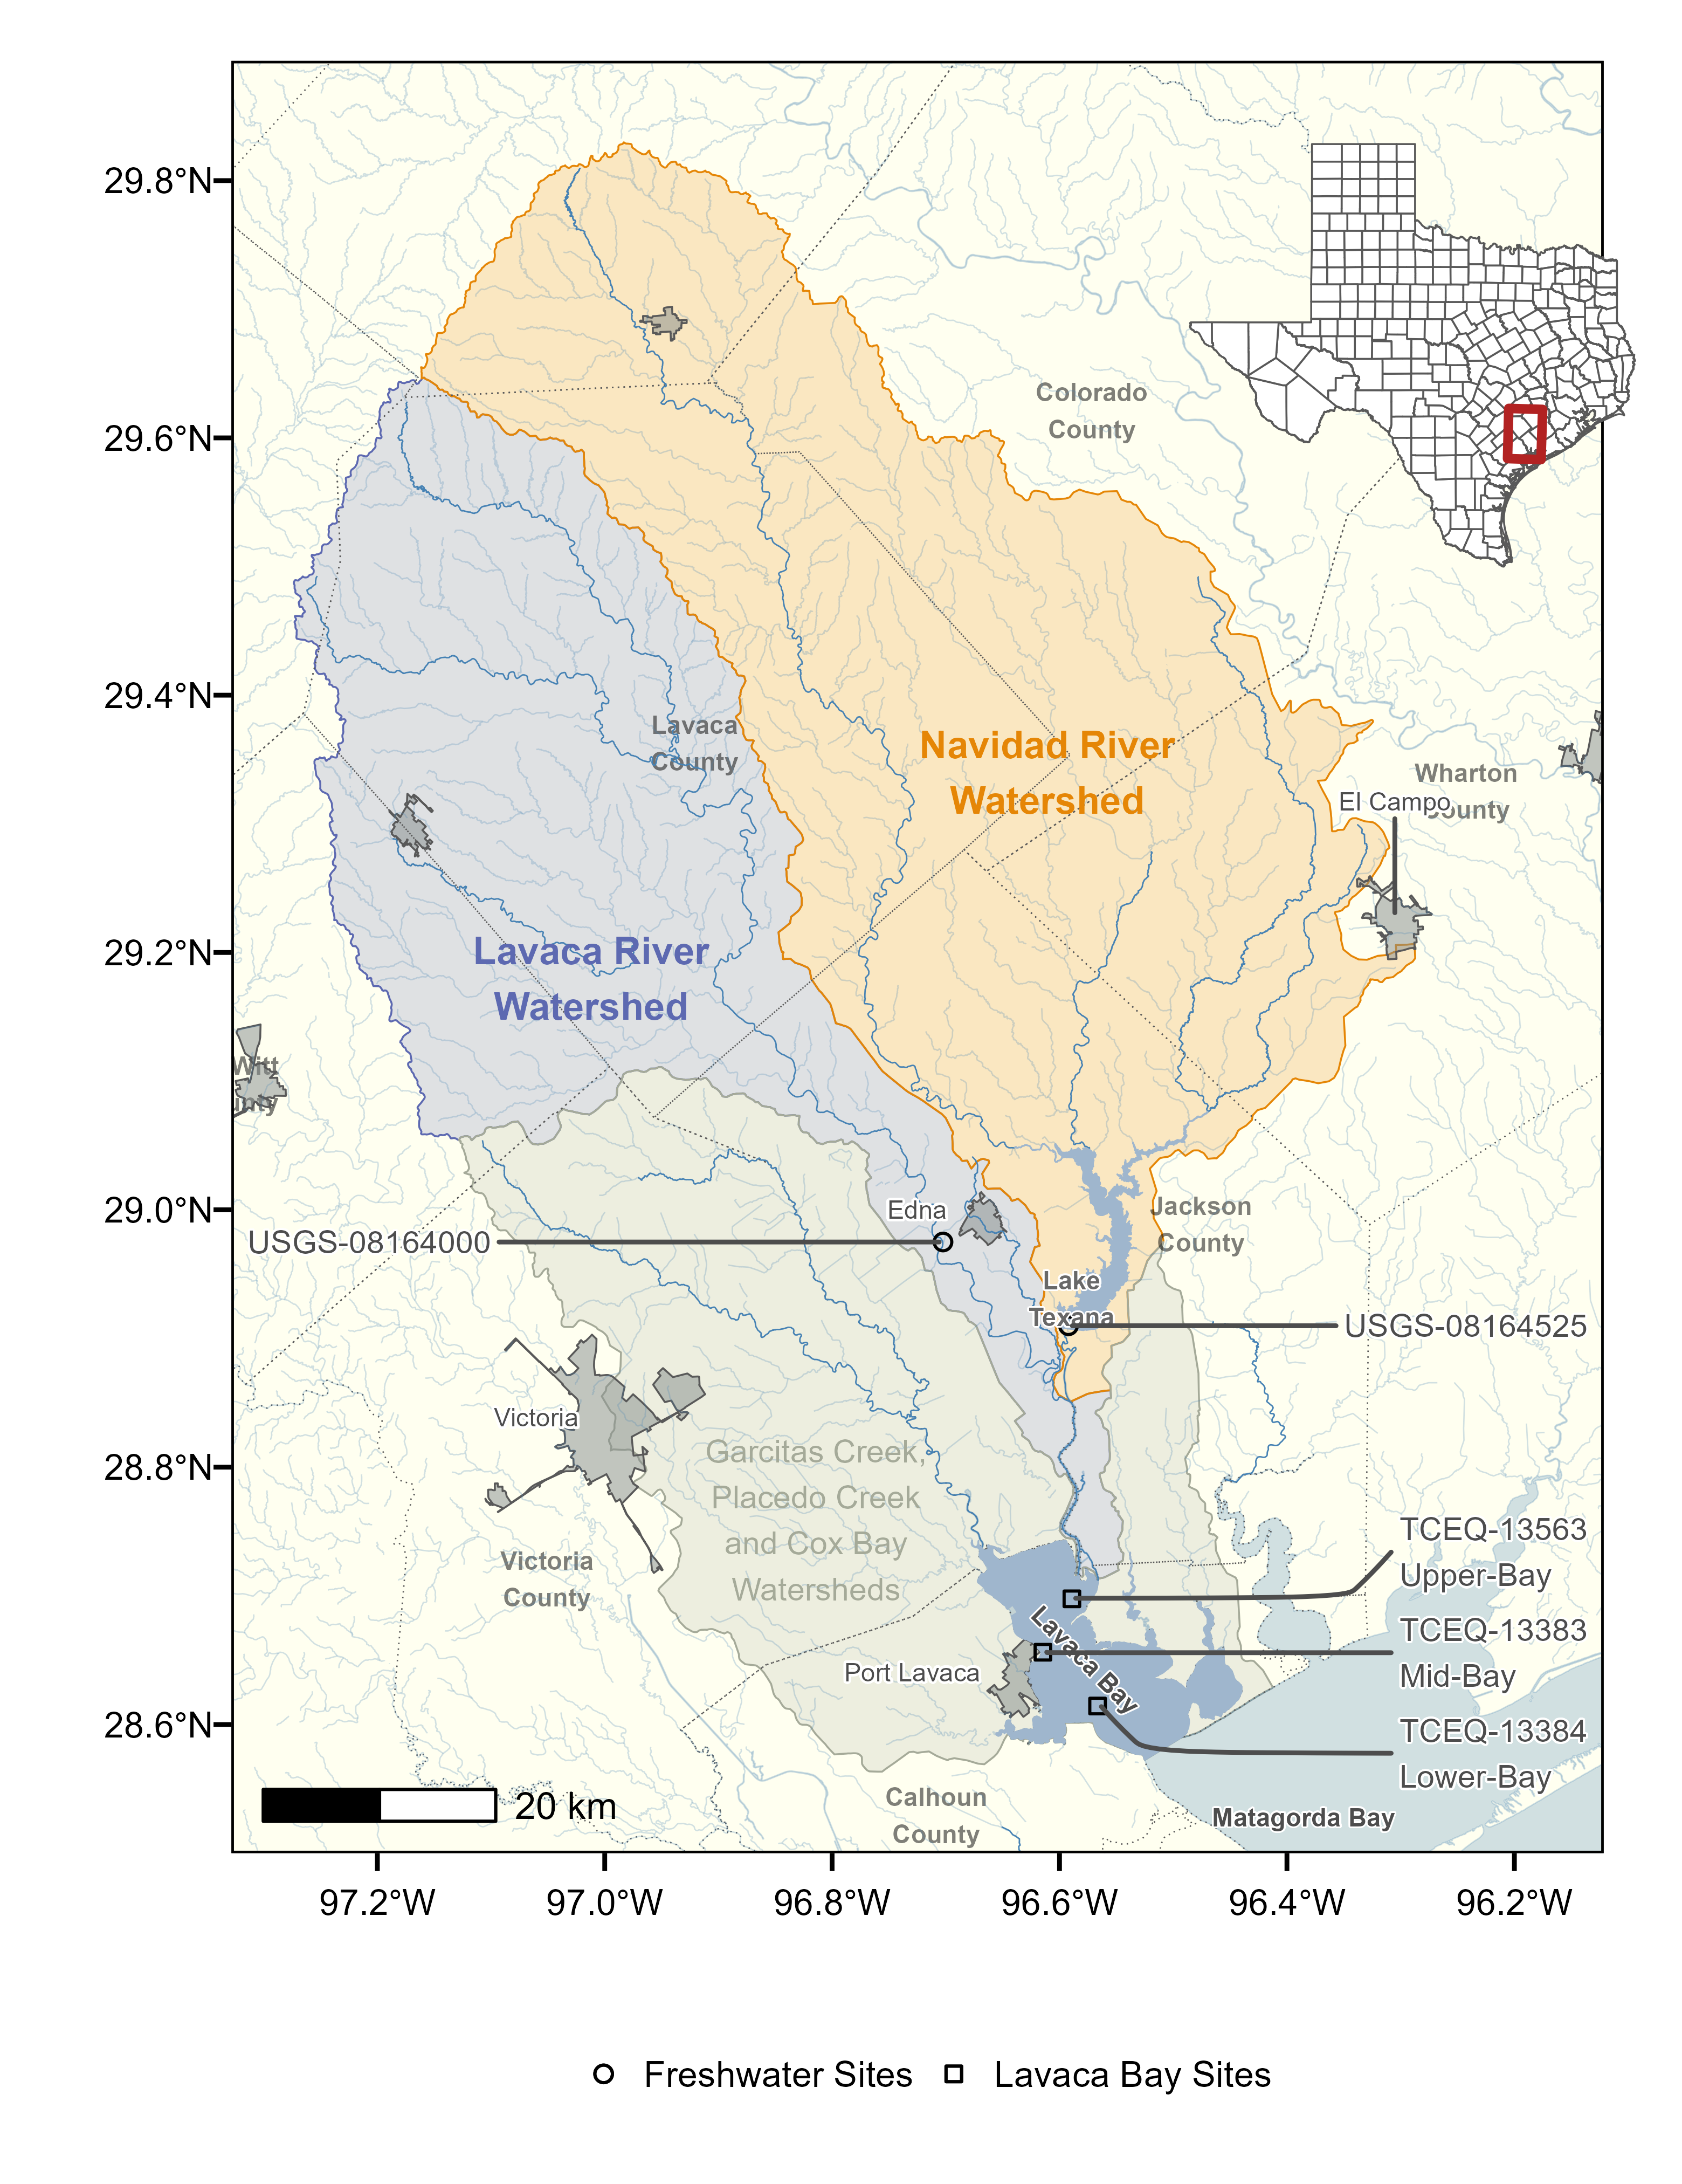
\includegraphics[width=5.2in,]{../fig1} 

}

\caption{Map of Lavaca Bay and the contribution watershed. The freshwater sites are the most downstream freshwater stream locations with water quality and streamflow data used for nutrient load models. Water quality concentration data at the three Lavaca Bay sites were used to assess relationships between freshwater flows, loads and estuary water quality.}\label{fig:fig1}
\end{figure}

Daily discharges for the Lavaca River (USGS-08164000,
Figure~\ref{fig:fig1}) were obtained from the United States Geologic
Survey (USGS) National Water Information System using the
\emph{dataRetrieval} R package
\citep{deciccoDataRetrievalPackagesDiscovering2022}. Gaged daily
discharges from the outlet of Lake Texana on the Navidad River
(USGS-0816425) were provided by the Texas Water Development Board (TWDB)
(April 21, 2022 email from R. Neupane, TWDB).

Water quality sample data for the two freshwater and three estuary
locations were obtained from the Texas Commission on Environmental
Quality (TCEQ) Surface Water Quality Monitoring Information System. Data
submitted through the system are required to be collected under Quality
Assurance Project Plans and lab method procedures outlined by the TCEQ's
procedures manual. The QAPP and procedures manuals ensure the consistent
collection and laboratory methods are applied between samples collected
by different entities and under different projects. All sites had
varying lengths of and availability of data. For freshwater locations,
TP from January 2000 through December 2020 and nitrate-nitrogen
(NO\textsubscript{3}) data from January 2005 through December 2020 were
downloaded (Table~\ref{tab:table1}). Less than 5-years of total nitrogen
and TKN concentration data were available at the freshwater sites and
deemed insufficient to develop load estimation models
\citep{horowitzEvaluationSedimentRating2003, snelderEstimationCatchmentNutrient2017}.
The three estuary sites included an upper Lavaca Bay site near the
outlet of the Lavaca River system (TCEQ-13563), a mid-Lavaca Bay site
(TCEQ-13383), and the lower Lavaca Bay site near the mouth of the Bay
(TCEQ-13384). For estuary locations, we obtained data for TP,
Nitrite+Nitrate (NO\emph{\textsubscript{x}}), TKN, chlorophyll-\emph{a},
and DO concentrations from January 2005 through December 2020
(Table~\ref{tab:table2}).

\begin{table}

\caption{\label{tab:table1}Summary of gauged streamflow and freshwater water quality samples between January 1, 2000 and December 31, 2020.}
\centering
\begin{tabular}[t]{llrrr}
\toprule
Station ID &   & Mean & SD & N\\
\midrule
USGS-08164000 & TP (mg/L) & \num{0.21} & \num{0.09} & 80\\
 & NO3 (mg/L) & \num{0.18} & \num{0.24} & 74\\
 & Mean Daily Streamflow (cfs) & \num{332.78} & \num{1667.47} & 7671\\
USGS-08164525 & TP (mg/L) & \num{0.20} & \num{0.08} & 81\\
 & NO3 (mg/L) & \num{0.29} & \num{0.26} & 62\\
 & Mean Daily Streamflow (cfs) & \num{666.14} & \num{2957.79} & 7671\\
\bottomrule
\end{tabular}
\end{table}

\begin{table}

\caption{\label{tab:table2}Summary of estuary water quality samples collected between January 1, 2005 and December 31, 2020.}
\centering
\begin{tabular}[t]{llrrr}
\toprule
Station ID &   & Mean & SD & N\\
\midrule
TCEQ-13383 & TP (mg/L) & \num{0.11} & \num{0.05} & 47\\
 & NOx (mg/L) & \num{0.07} & \num{0.15} & 51\\
 & TKN (mg/L) & \num{0.94} & \num{0.49} & 45\\
 & Chlorophyll-a (ug/L) & \num{9.43} & \num{5.31} & 47\\
 & DO (mg/L) & \num{7.22} & \num{1.35} & 55\\
TCEQ-13384 & TP (mg/L) & \num{0.08} & \num{0.03} & 51\\
 & NOx (mg/L) & \num{0.06} & \num{0.08} & 52\\
 & TKN (mg/L) & \num{0.76} & \num{0.40} & 48\\
 & Chlorophyll-a (ug/L) & \num{8.22} & \num{6.44} & 46\\
 & DO (mg/L) & \num{7.51} & \num{1.32} & 54\\
TCEQ-13563 & TP (mg/L) & \num{0.13} & \num{0.06} & 50\\
 & NOx (mg/L) & \num{0.09} & \num{0.13} & 53\\
 & TKN (mg/L) & \num{0.94} & \num{0.37} & 49\\
 & Chlorophyll-a (ug/L) & \num{9.67} & \num{5.33} & 49\\
 & DO (mg/L) & \num{7.91} & \num{1.34} & 56\\
\bottomrule
\end{tabular}
\end{table}

\hypertarget{estimating-watershed-based-nutrient-loads}{%
\subsection{Estimating Watershed Based Nutrient
Loads}\label{estimating-watershed-based-nutrient-loads}}

Estimates of NO\textsubscript{3} and TP loads at the Lavaca River
(USGS-08164000) and the outlet of Lake Texana on the Navidad River
(USGS-08164525) were developed using GAMs relating nutrient
concentration to river discharge, season, and time. Separate models were
fit at each station for each parameter and used to predict nutrient
concentrations for each day in the study period. GAMs were fit using the
\emph{mgcv} package in R which makes available multiple types of smooth
functions with automatic smoothness selection
\citep{woodFastStableRestricted2011}. The general form of the model
related NO\textsubscript{3} or TP concentration to a long term tend,
season, streamflow, and two different antecedent discharge terms, shown
in Eq. \ref{eq1}:

\begin{align}
g(\mu) &= \alpha + f_1(ddate) + f_2(yday) + f_3(log1p(Q)) + f_4(ma) + f_5(fa), \nonumber \\
y &\sim \mathcal{N}(\mu,\,\sigma^{2})
\label{eq1}
\end{align}

where \(\mu\) is the conditional expected NO\textsubscript{3} or TP
concentration, \(g()\) is the log-link, \(\alpha\) is the intercept,
\(f_n()\) are smoothing functions. \(y\) is the response variable
(NO\textsubscript{3} or TP concentration) modeled as normally
distributed with mean \(\mu\) and standard deviation \(\sigma\).
\emph{ddate} is the date converted to decimal notation, \emph{yday} is
numeric day of year (1-366), and \emph{log1p(Q)} is the natural log of
mean daily streamflow plus 1.

Moving average (\emph{ma}) is an exponentially smoothed moving average
that attempts to incorporate the influence of prior streamflow events on
concentration at the current time period
\citep{wangLoadEstimationUncertainties2011, kuhnertQuantifyingTotalSuspended2012, zhang_improving_2017},
using Eq. \ref{eq2}:

\begin{align}
ma(\delta) &= d{\kappa_{i-1}}+(1-\delta)\hat{q}_{i-1}, \nonumber \\
\kappa_{i} &=\sum_{m=1}^{i}\hat{Q}_m
\label{eq2}
\end{align}

where \(\delta\) is the discount factor (here, set equal to 0.95),
\(\kappa_i\) is the cumulative flow (\emph{Q}) up to the \emph{i}th day.

Flow anomaly (\emph{fa}) is a unitless term that represents how wet or
dry the current time period is from a previous time period
\citep{vecchiaTrendsConcentrationsUse2009, zhang_improving_2017}.
Long-term flow anomaly (\emph{ltfa}) is the streamflow over the previous
year relative to the entire period \citep{zhang_improving_2017} and
calculated using Eq. \ref{eq3}:

\begin{equation}
ltfa(t) = \bar{x}_{1\,year}(t) - \bar{x}_{entire\,period}
\label{eq3}
\end{equation}

and the short-term flow anomaly (\emph{stfa}) calculated as the current
day flow compared to the preceding 1-month streamflow using \ref{eq4}:

\begin{equation}
stfa(t) = x_{current\,day}(t) - \bar{x}_{1\,month}(t)
\label{eq4}
\end{equation}

where \(x\) are the averages of log-transformed streamflow over the
antecedent period (\emph{1-year}, \emph{1-month}, etc.) for time
\emph{t}. We used \emph{ltfa} in NO\textsubscript{3} models and
\emph{stfa} in TP models based on previous work demonstrating major
improvements in NO\textsubscript{x} regression models that incorporated
\emph{ltfa} and moderate improvements in TP regression models that
incorporated \emph{stfa} \citep{zhang_improving_2017}.

The calculation of model terms for the Lake Texana site were modified
because daily loads are not a function of natural stream flow processes
alone, but of dam releases and nutrient concentrations at the discharge
point of the lake. \emph{Q}, \emph{ma}, and \emph{fa} terms were
calculated based on total gaged inflow from the 4 major tributaries to
the lake. Thin-plate regression splines were used for \emph{ddate},
\emph{log1p(Q)}, \emph{fa}, and \emph{ma}. A cyclic cubic regression
spline was used for \emph{yday} to ensure the ends of the spline match
(day 1 and day 366 are expected to match). First order penalties were
applied to the smooths of flow-based variables which penalize departures
from a flat function to help constrain extrapolations for high flow
measurements.

Left-censored data were not uncommon in this dataset. Several methods
are available to account for censored data. We transformed left-censored
nutrient concentrations to one-half the detection limit. Although this
simple approach can introduce bias
\citep{hornungEstimationAverageConcentration1990}, we considered it
acceptable because high concentrations and loadings are associated with
high-flow events and low-flow/low-concentration events will account for
a small proportion of total loadings \citep{mcdowell_implications_2021}.

Daily loads were estimated as the predicted concentration multiplied by
the daily streamflow. For the Navidad River (USGS-08164525) site, daily
loads at the dam were calculated from the discrete daily concentration
at the discharge point of the lake and corresponding reported daily
discharge from the dam. Flow-normalized loads were estimated similar to
WRTDS by setting flow-based covariates on each day of the year equal to
each of the historical values for that day of the year over the study
period \citep{hirschWeightedRegressionsTime2010}. The flow-normalized
estimate was calculated as the mean of all the predictions for each day
considering all possible flow values. Standard deviations and credible
intervals were obtained by drawing samples from the multivariate normal
posterior distribution of the fitted GAM
\citep{woodConfidenceIntervalsGeneralized2006, marraCoveragePropertiesConfidence2012, mcdowell_implications_2021}.
Uncertainty in loads were calculated as 90\% credible intervals
estimated by drawing 1000 realizations of parameter estimates from the
multivariate normal posterior distribution of the model parameters. GAM
performance was evaluated using repeated 5-fold cross validation
\citep{burmanComparativeStudyOrdinary1989} and average Nash-Sutcliffe
Efficiency (NSE), Pearson sample correlation (\emph{r}) and percent bias
(PBIAS) metrics across folds were calculated for each model.

\hypertarget{linking-estuary-water-quality-to-hydrology-and-nutrient-loads}{%
\subsection{Linking Estuary Water Quality to Hydrology and Nutrient
Loads}\label{linking-estuary-water-quality-to-hydrology-and-nutrient-loads}}

To test if changes in freshwater inflow and nutrient loading had
explanatory effect on changes in estuary water quality a series of GAM
models were fit at each site relating parameter concentration to
temporal trends (\citep{eq-eq5}), temporal trends and inflow
(\citet{eq-eq6}), and temporal trends, inflow, and nutrient loads
(\citet{eq-eq7}): \begin{align}
g(\mu) &= \alpha + f_1(ddate) + f_2(yday), \label{eq5} \\
g(\mu) &= \alpha + f_1(ddate) + f_2(yday) + f_3(Q), \label{eq6} \\
g(\mu) &= \alpha + f_1(ddate) + f_2(yday) + f_3(Q) + f_4(Load) \label{eq7}
\end{align}

where \(\mu\) is the conditional expected response (nutrient
concentration), \(g()\) is the log link, and response variable was
modeled as Gamma distributed with mean \(\mu\) and scale \(\lambda\).
\(f_1(ddate)\) is decimal date smoothed with a thin-plate regression
spline, \(f_2(yday)\) is the numeric day of year smoothed with a cyclic
cubic regression spline, \(f_3(Q)\) is mean daily inflow (the combined
measurements from Lavaca River and Navidad River) and \(f_4(Load)\) is
the total NO\textsubscript{3} or TP watershed load. The set of models
specified for each water quality response are in Table~\ref{tab:table3}.

\begin{table}

\caption{\label{tab:table3}Set of GAM models specified for each water quality parameter response.}
\centering
\begin{tabular}[t]{lll}
\toprule
Parameter & Model & Model Terms\\
\midrule
 & Temporal & s(ddate) + s(yday)\\

 & Flow & s(ddate) + s(yday) + s(Q)\\

\multirow{-3}{*}{\raggedright\arraybackslash TP} & Flow+Load & s(ddate) + s(yday) + s(Q) + s(TP Load)\\
\cmidrule{1-3}
 & Temporal & s(ddate) + s(yday)\\

 & Flow & s(ddate) + s(yday) + s(Q)\\

\multirow{-3}{*}{\raggedright\arraybackslash NO\textsubscript{x}} & Flow+Load & s(ddate) + s(yday) + s(Q) + s(NO\textsubscript{3} Load)\\
\cmidrule{1-3}
 & Temporal & s(ddate) + s(yday)\\

 & Flow & s(ddate) + s(yday) + s(Q)\\

\multirow{-3}{*}{\raggedright\arraybackslash Chlorophyll-\textit{a}} & Flow+Load & s(ddate) + s(yday) + s(Q) + s(TP Load) + s(NO\textsubscript{3} Load)\\
\cmidrule{1-3}
 & Temporal & s(ddate) + s(yday)\\

 & Flow & s(ddate) + s(yday) + s(Q)\\

\multirow{-3}{*}{\raggedright\arraybackslash Dissolved Oxygen} & Flow+Load & s(ddate) + s(yday) + s(Q) + s(TP Load) + s(NO\textsubscript{3}  Load)\\
\cmidrule{1-3}
 & Temporal & s(ddate) + s(yday)\\

\multirow{-2}{*}{\raggedright\arraybackslash TKN} & Flow & s(ddate) + s(yday) + s(Q)\\
\bottomrule
\end{tabular}
\end{table}

Because streamflow and nutrient loads are tightly correlated, freshwater
inflow can mask signals from nutrient loads alone. Following the
methodology implemented by
\citet{murphyNutrientImprovementsChesapeake2022}, both streamflow and
nutrient loads were prepossessed to account for season and flow.
Freshwater inflow and nutrient loads were replaced by seasonally
adjusted log transformed inflow and flow-adjusted log transformed
nutrient loads obtained by fitting a GAM relating season (day of year)
to log transformed daily freshwater inflow values and a GAM relating log
transformed NO\textsubscript{3} or TP loads to log transformed daily
inflow.Response residuals from the respective GAM models were used as
\emph{Q} and \emph{Load} in Eq.~\ref{eq6} and Eq.~\ref{eq7}.

This study used an information theoretic approach to evaluate if
nutrient loads and/or freshwater inflows provided evidence of effects on
water quality concentrations in Lavaca Bay. Model probabilities were
calculated and compared using the AIC\textsubscript{c} scores between
each group of temporal, flow, and flow+load models
\citep{burnhamAICModelSelection2011}. Improvements in model
probabilities provide evidence that the terms explain additional
variation in the response variable. If model probabilities were tied,
there wasn't evidence the more complicated model explains additional
variation in water quality.

\hypertarget{sec3}{%
\section{Results}\label{sec3}}

\hypertarget{watershed-nutrient-loads}{%
\subsection{Watershed Nutrient Loads}\label{watershed-nutrient-loads}}

Using evaluation criteria recommended by
\citet{moriasiHydrologicWaterQuality2015}, predictive performance of
nutrient loading GAMs ranged from ``satisfactory'' to ``very good''
based on median NSE, \emph{r}, and PBIAS metrics calculated using 5-fold
cross validation. Median goodness-of-fit metrics for NO\textsubscript{3}
models in the Lavaca River were 0.34 NSE, 0.70 \emph{r}, and 2.00 PBIAS.
Navidad River NO\textsubscript{3} models appeared to perform slightly
better with 0.48 NSE and 0.87 \emph{r} but with higher bias at 10.90
PBIAS. Generally, TP models performed better than NO\textsubscript{3}
models. Median goodness-of-fit metrics for TP in the Lavaca River were
0.81 NSE, 0.93 \emph{r}, and -7.20 PBIAS. Navidad River TP models has
similar performance with 0.91 NSE, 0.99 \emph{r}, and -3.30 PBIAS.
Density plots of metrics show similar distribution of values between
sites for the same parameter, with the exception \emph{r} values for
NO\textsubscript{3} loads where Lavaca River had a much larger variance
in values compared to the Navidad River (Figure~\ref{fig:fig2}). TP GAMS
had higher average NSE and \emph{r} values and lower variance in metric
values compared to NO\textsubscript{3}.

\begin{figure}

{\centering 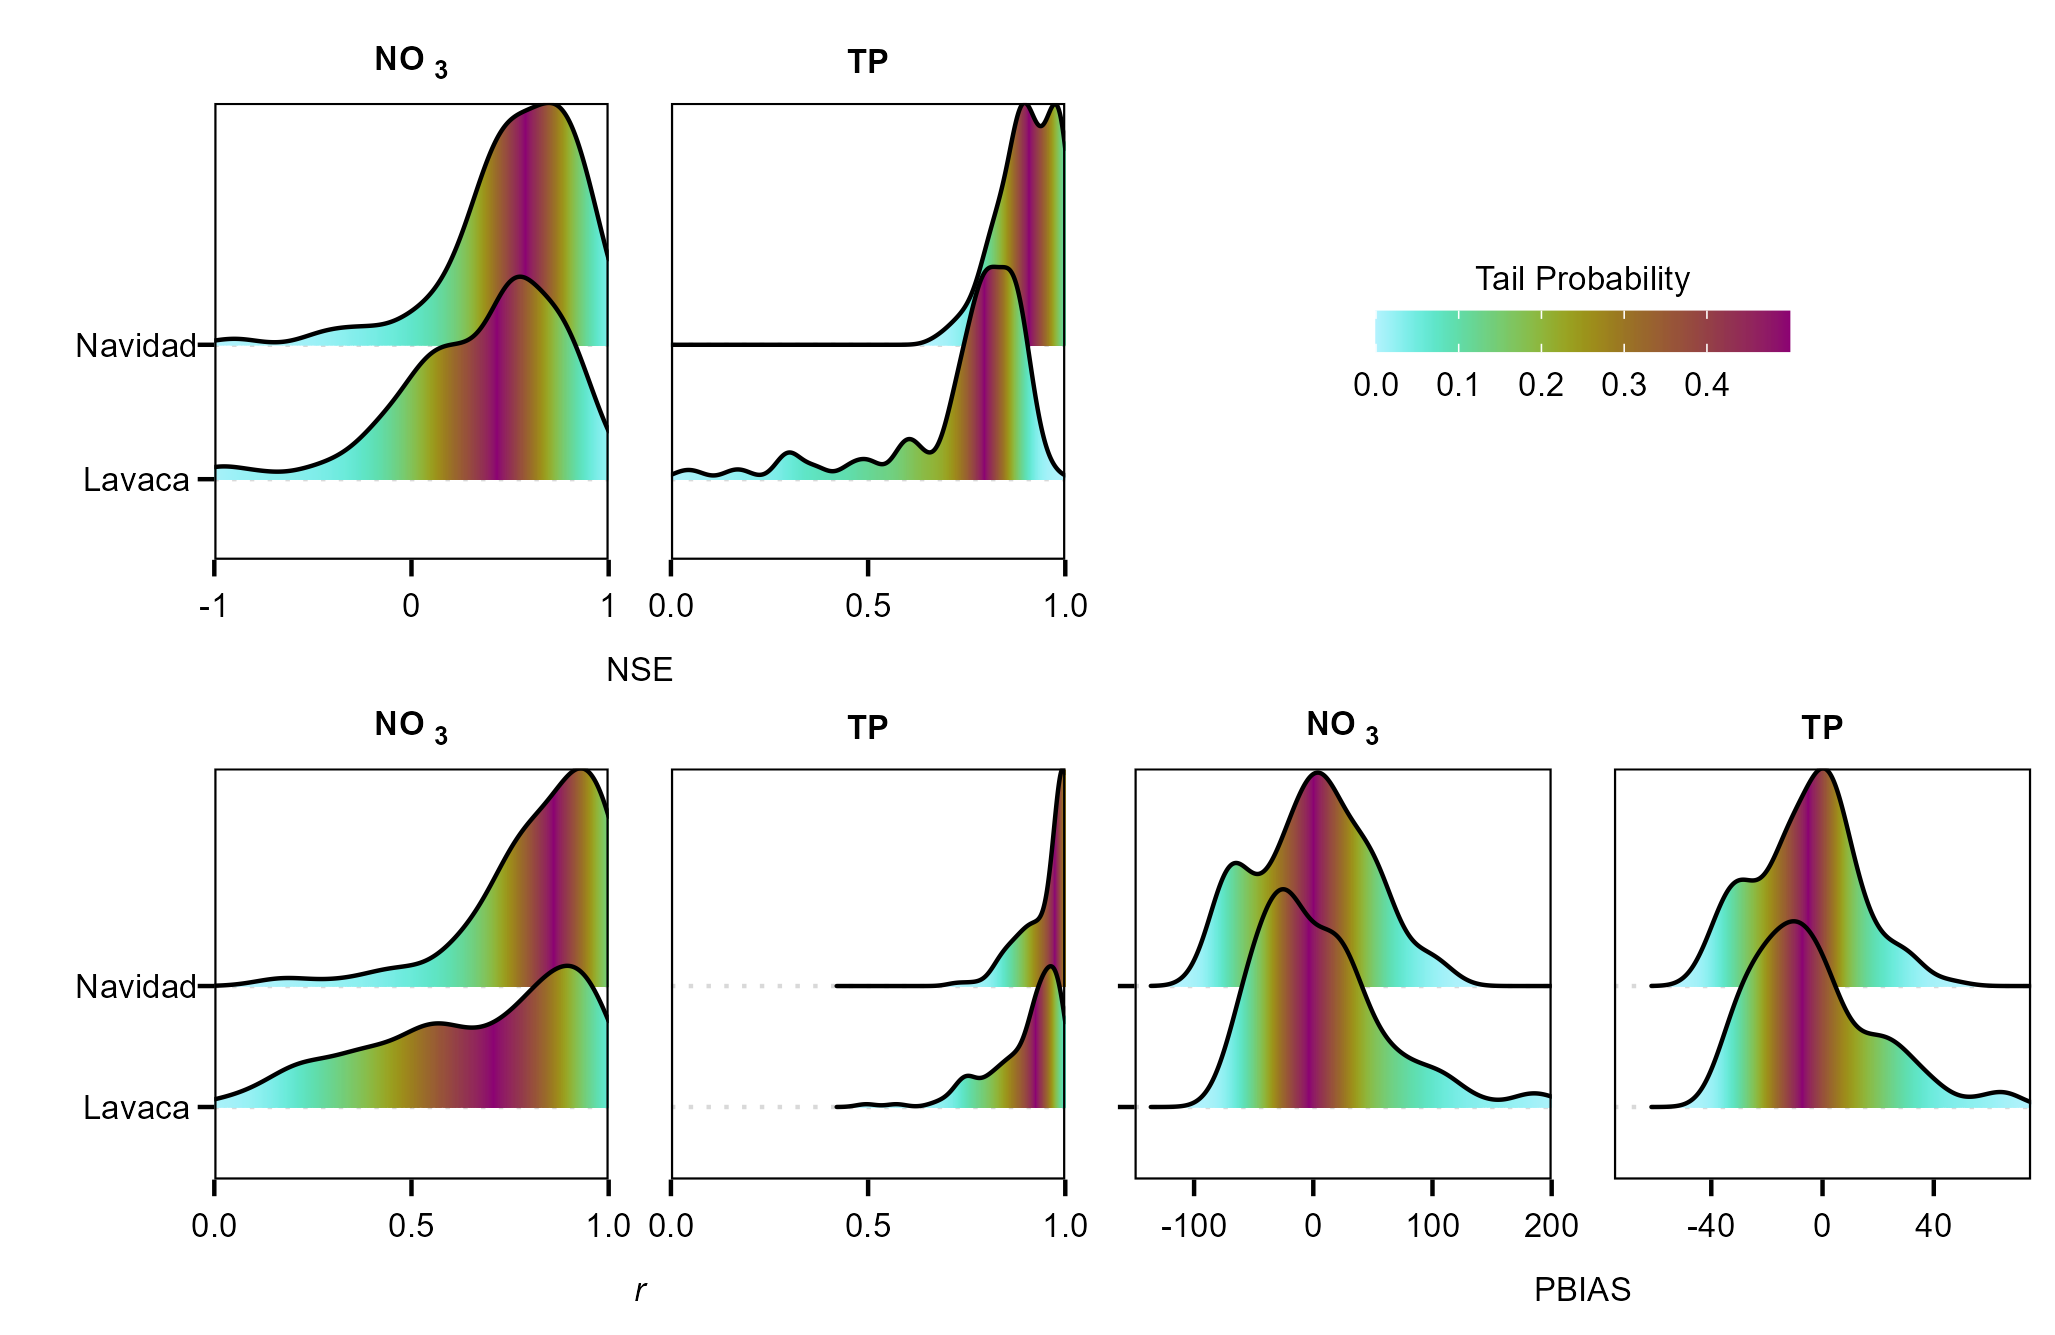
\includegraphics[width=1\linewidth,]{Schramm-2023-05-AS_files/figure-latex/fig2-1} 

}

\caption{Density plots of goodness-of-fit metrics (NSE, \textit{r}, and PBIAS) from repeated 5-fold cross validation between predicted nutrient loads from GAM models and measured nutrient loads. Color indicates the tail probability calculated from the empirical cumulative distribution of the goodness-of-fit metrics.}\label{fig:fig2}
\end{figure}

Predicted annual NO\textsubscript{3} and TP loads show considerable
variation, generally following patterns in discharge
(Figures~\ref{fig:fig3}, \ref{fig:fig4}). Flow-normalized TP loads at
both sites and flow-normalized NO\textsubscript{3} loads in the Lavaca
River indicated watershed based loads did not change much over time when
accounting for variation driven by streamflow (Figure~\ref{fig:fig3}).
Flow-normalized loads in the Lavaca River showed small variation over
time with some decreases in NO\textsubscript{3} loads since 2013.

\begin{figure}

{\centering 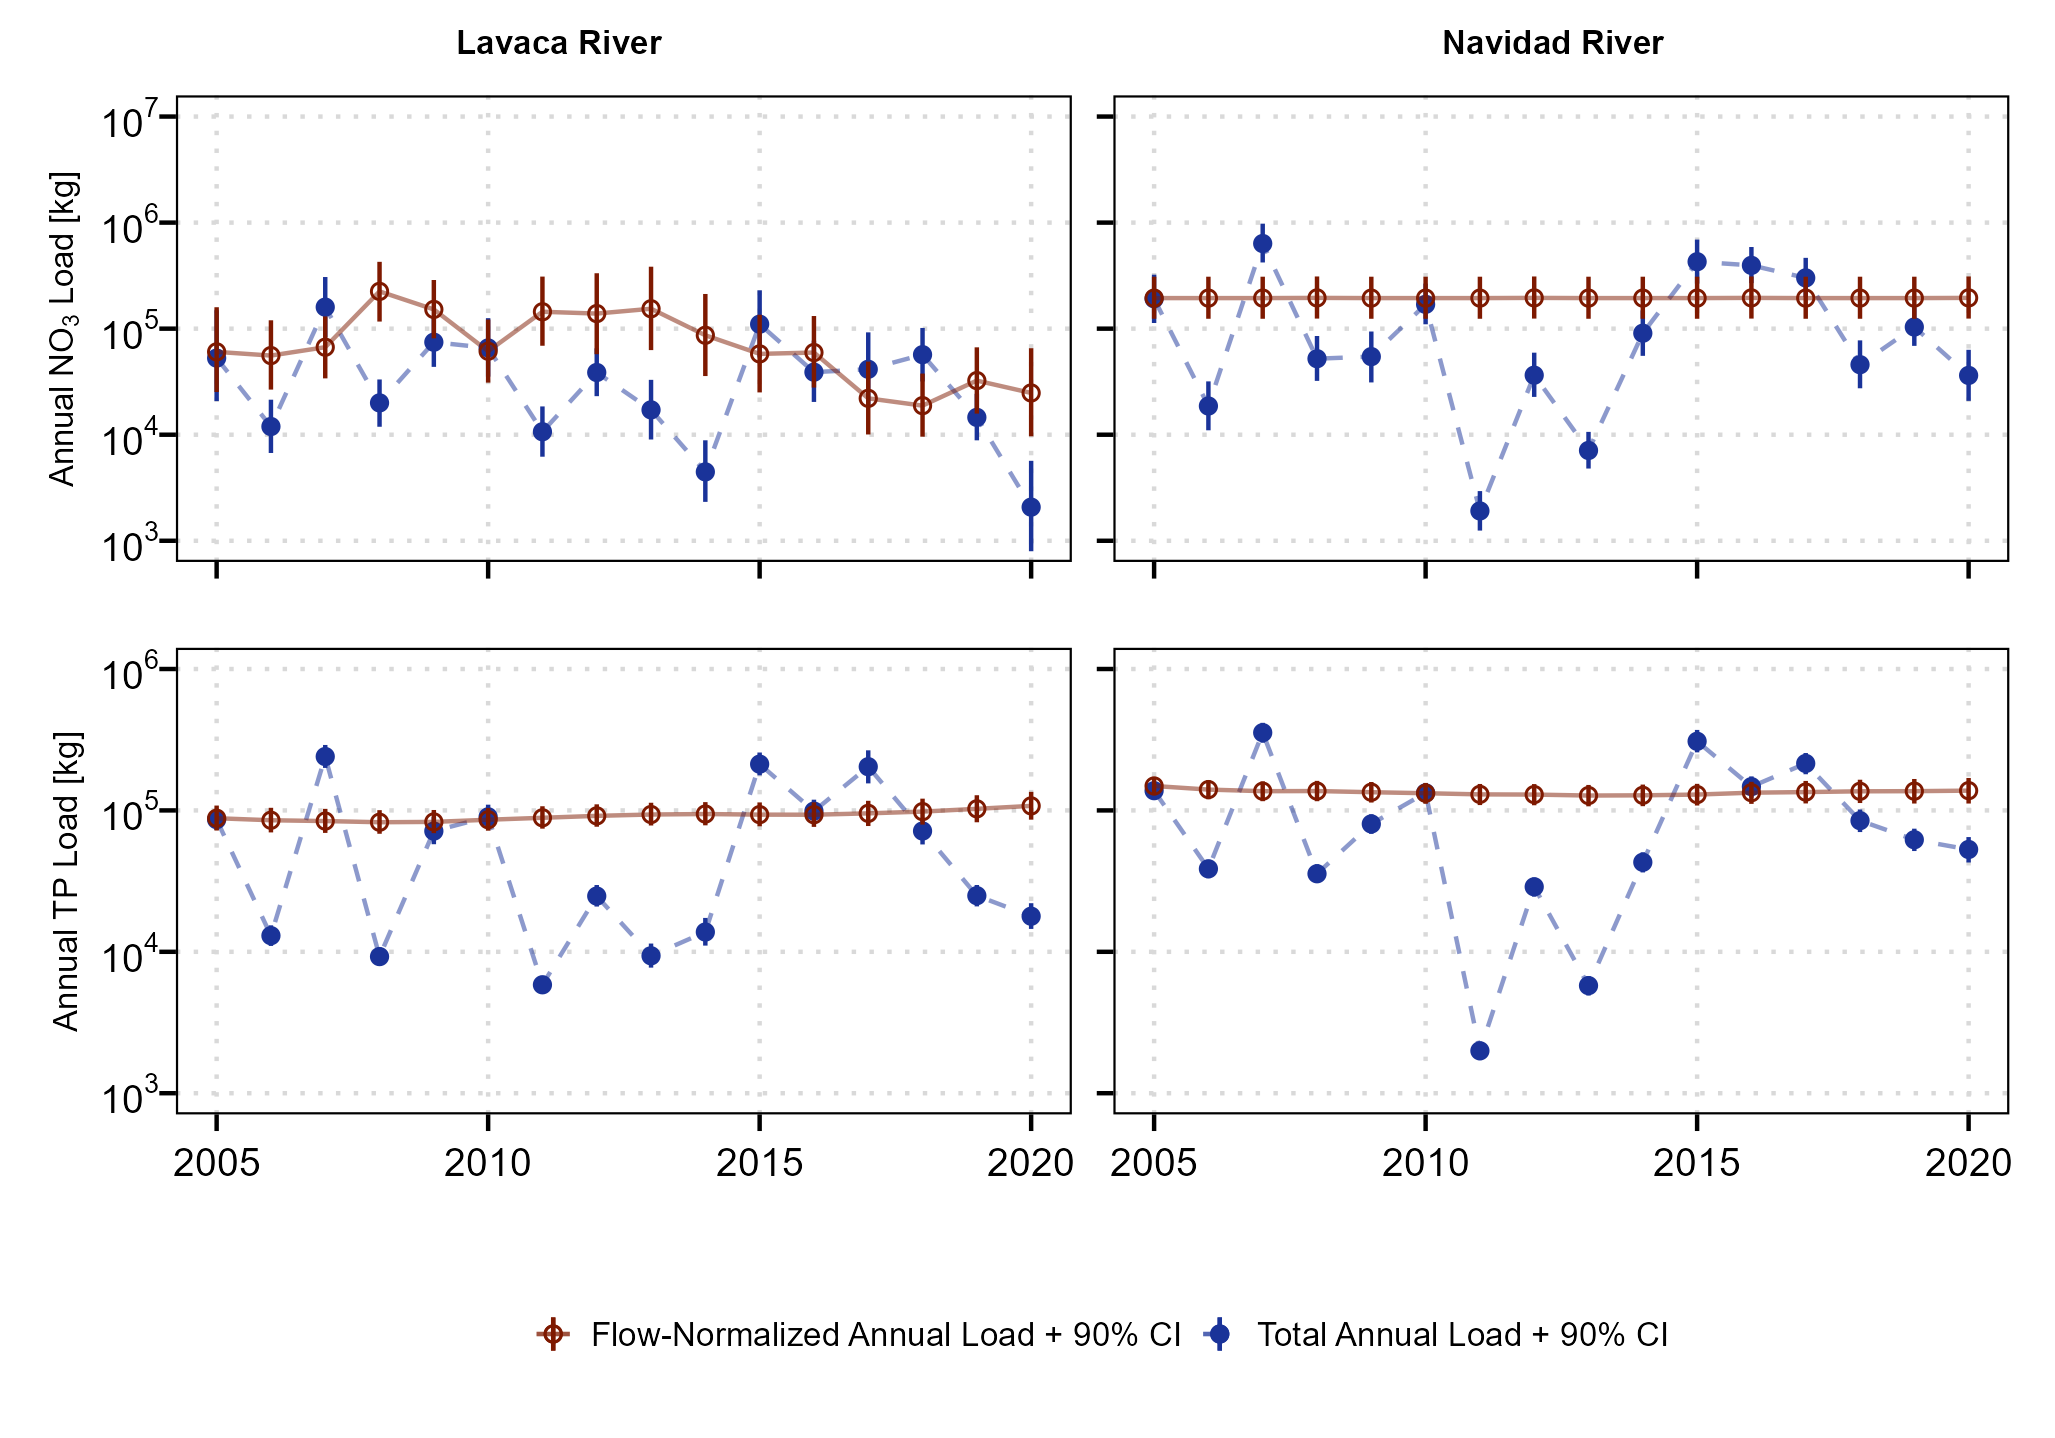
\includegraphics[width=1\linewidth,]{Schramm-2023-05-AS_files/figure-latex/fig3-1} 

}

\caption{Aggregated estimated annual and flow-normalized annual NO~3~ and TP loads for USGS-08164000 and USGS-08164525.}\label{fig:fig3}
\end{figure}

Aggregated across both sites, the mean annual NO\textsubscript{3} load
2005 through 2020 was 205,405 kg (126,867 kg - 341,569 kg, 90\% CI).
Annual NO\textsubscript{3} loads ranged from 12,574 kg in 2011 to
794,510 kg in 2007. Total annual TP loads ranged from 7,839 kg in 2011
to 595,075 kg in 2007. Mean annual TP loading from 2005 through 2020 was
182,673 kg (152,227 kg - 219,310 kg, 90\% CI). On average, the Navidad
River accounted for 68\% of NO\textsubscript{3} loads and 59\% of TP
loads from 2005 through 2020. However, during periods of extreme drought
the Lavaca River became the primary source of nutrient loading in the
watershed with the Navidad River only accounting for 15\% and 25\% of
NO\textsubscript{3} and TP loads in 2011 (Figure~\ref{tab:fig4}).

\begin{figure}

{\centering 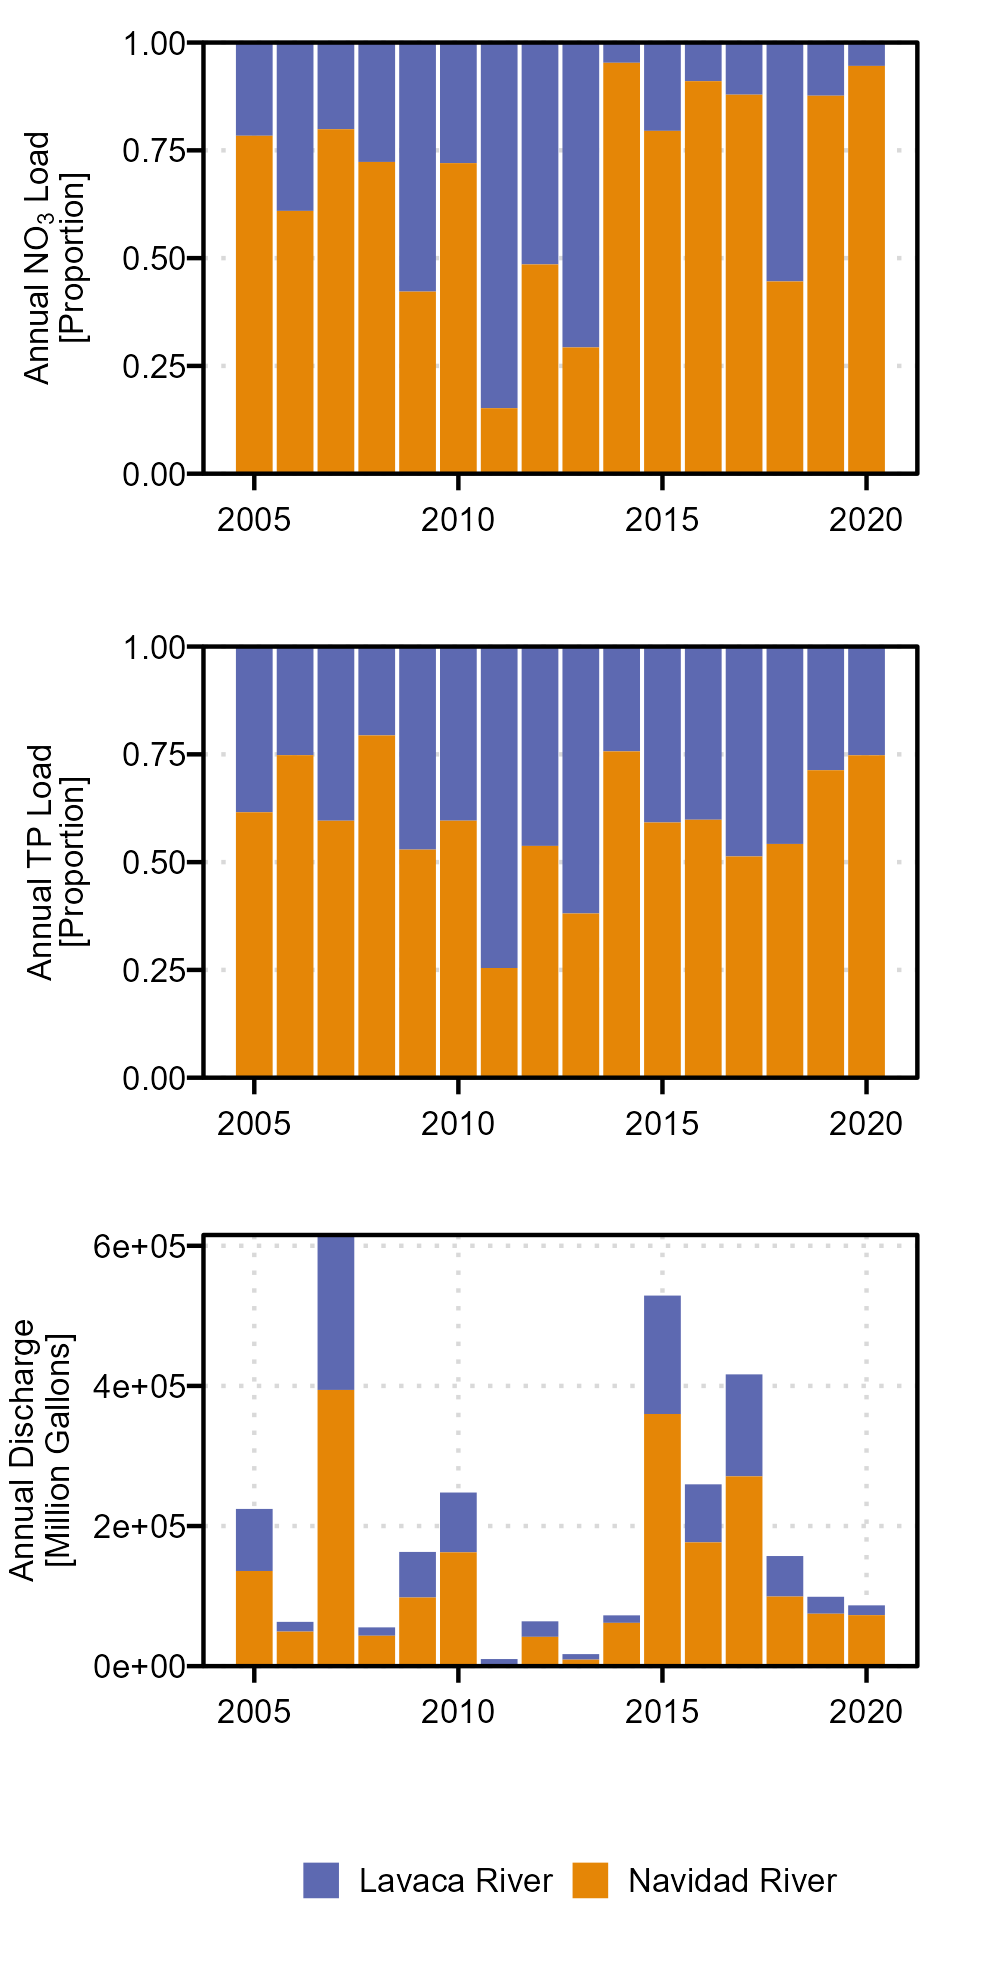
\includegraphics[width=0.5\linewidth,]{Schramm-2023-05-AS_files/figure-latex/fig4-1} 

}

\caption{Comparison of delivered annual loads and annual discharge at the Lavaca (USGS-08164000) and Navidad (USGS-08164525) Rivers.}\label{fig:fig4}
\end{figure}

\hypertarget{linkages-between-water-quality-and-watershed-flows-and-loads}{%
\subsection{Linkages Between Water Quality and Watershed Flows and
Loads}\label{linkages-between-water-quality-and-watershed-flows-and-loads}}

GAMs did not identify significant changes in TP or DO concentrations at
any of the Lavaca Bay sites from 2005 through 2020
(Figure~\ref{fig:fig5}). The upper-bay site, TCEQ-13563, had a linear
increase in NO\textsubscript{x} concentration and and decrease in
chlorophyll-\emph{a} from 2005 through 2014. The mid-bay site,
TCEQ-13383, showed a periodic pattern in NO\textsubscript{x}
concentration that appeared similar to precipitation/inflow patterns, as
well as a post 2011 increase in TKN concentrations. No significant
long-term trends in concentrations were identified by GAMs for the
lower-bay TCEQ-13384 site.

\begin{figure}

{\centering 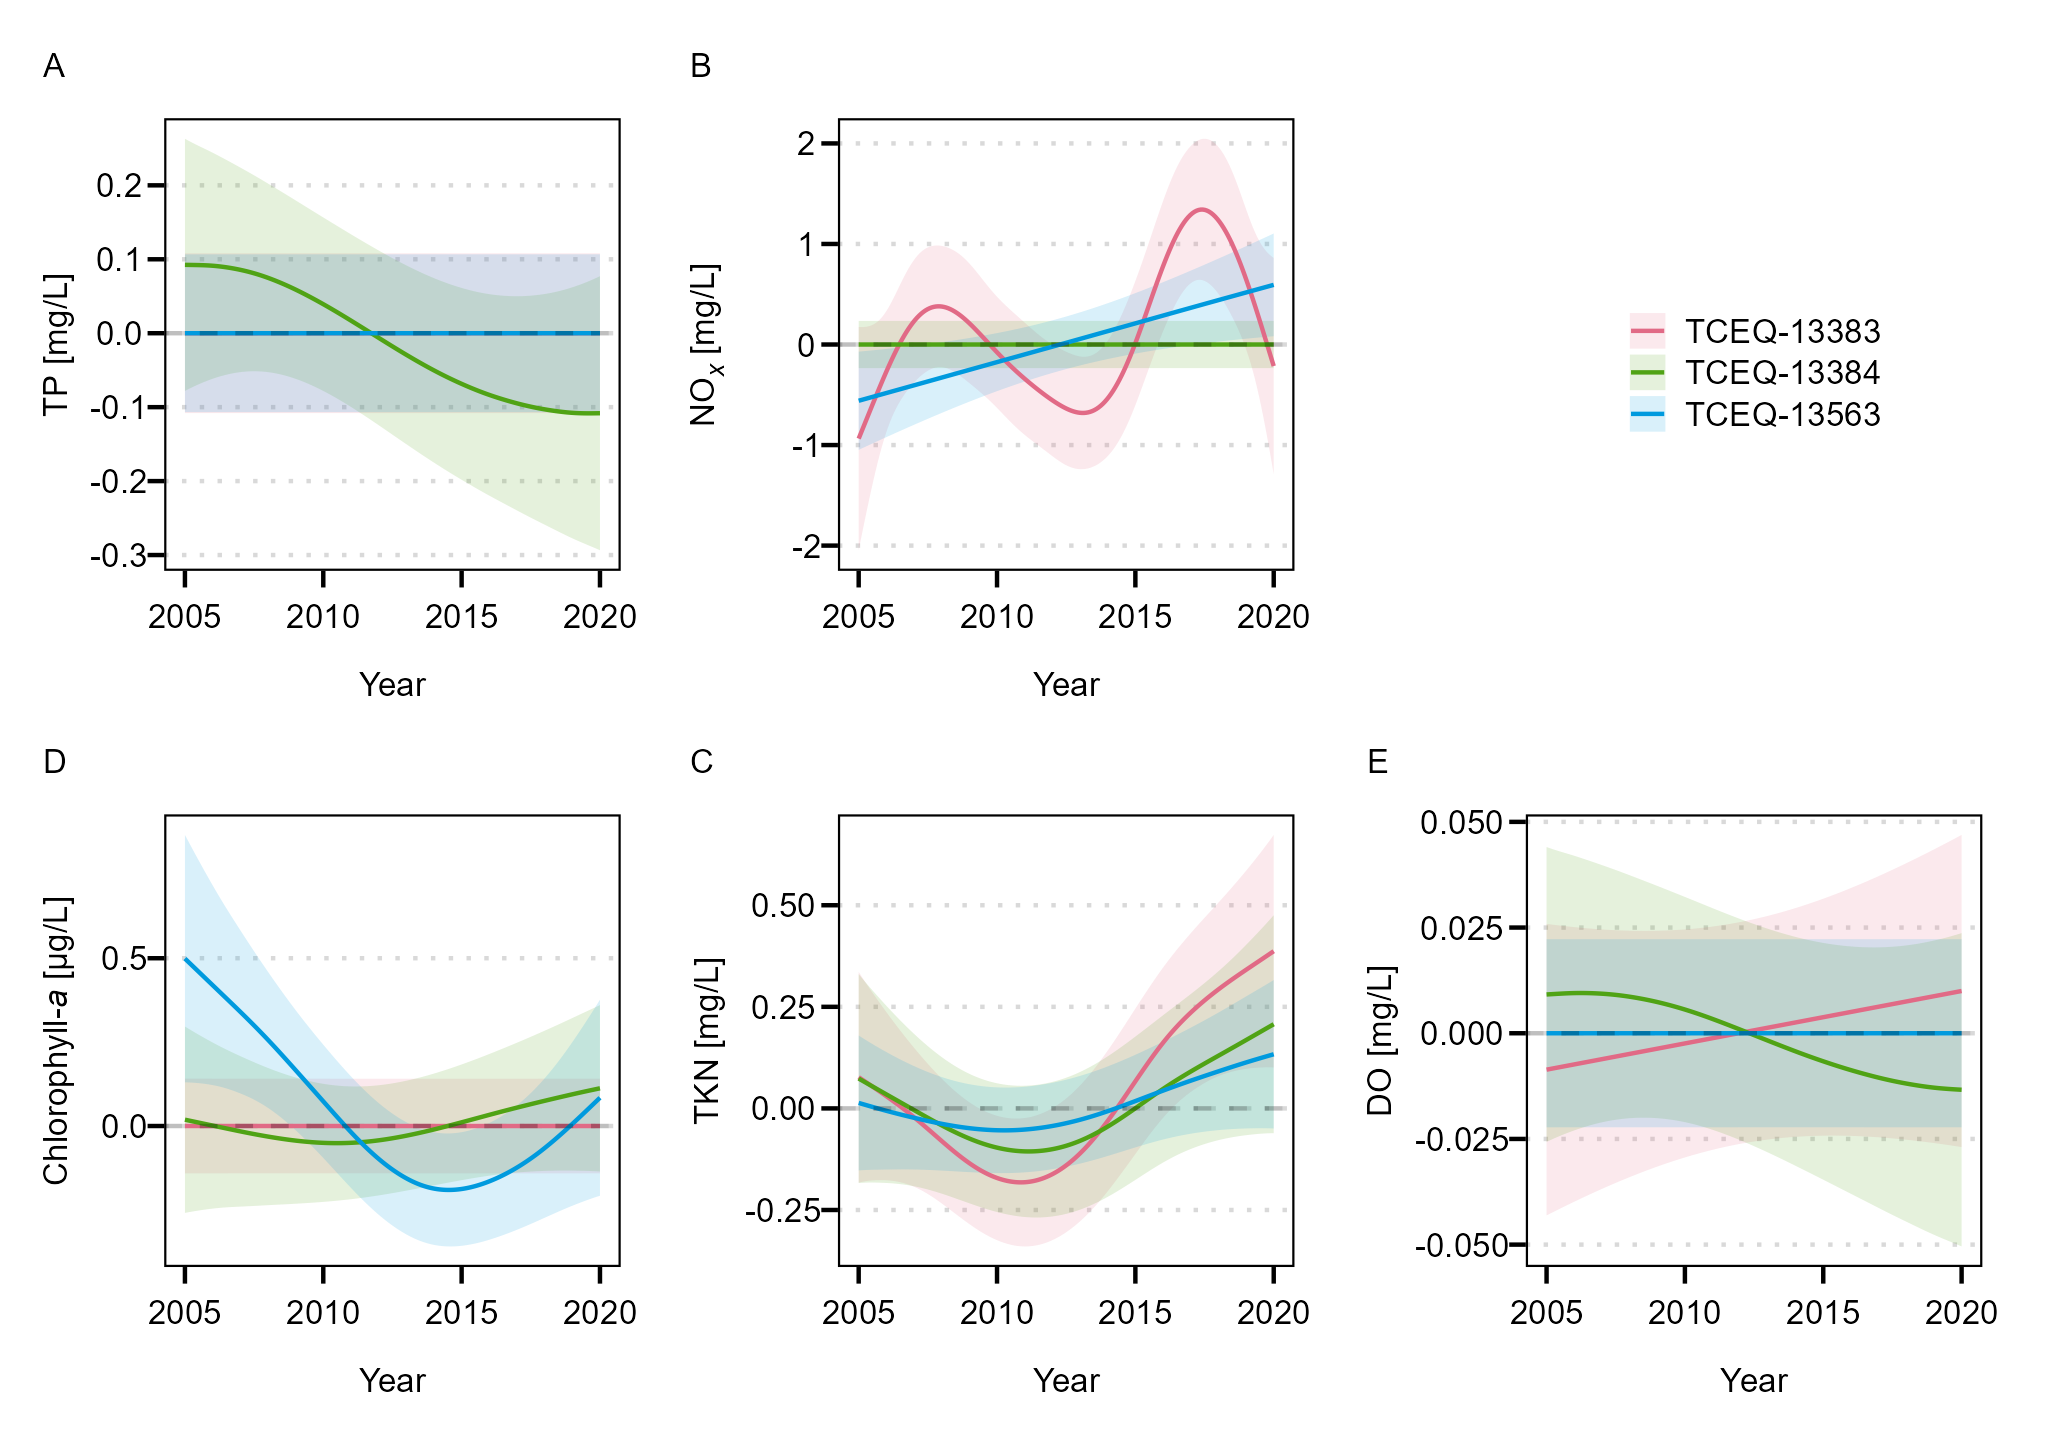
\includegraphics[width=1\linewidth,]{Schramm-2023-05-AS_files/figure-latex/fig5-1} 

}

\caption{Smoothed temporal trend component for water quality paramaters obtained from temporal estuary GAMs.}\label{fig:fig5}
\end{figure}

Freshwater inflow provided additional explanation for changes in TP and
NO\textsubscript{\emph{x}} concentration at all of the Lavaca Bay sites
according to AIC\textsubscript{c} and model probability values
(Table~\ref{tab:table4}). TCEQ-13563, the site closest to the river
outlet, was the only site that had improvements in the explanations of
DO and TKN concentration with the inclusion of inflow. Both TCEQ-13563
and TCEQ-13383, the mid-bay site, saw improvements in explanations for
variations in chlorophyll-\emph{a} with the inclusion of freshwater
inflow. The addition of nutrient loads (both TP and NO\textsubscript{3})
terms did not provide additional explanation for changes in
chlorophyll-\emph{a} or DO concentrations. Inclusion of TP loads
provided additional explanation of TP concentrations at the upper- and
mid-bay sites, TCEQ-13563 and TCEQ-13383. Inclusion of
NO\textsubscript{3} loads only provided marginal improvements in the
explanation of NO\textsubscript{\emph{X}} concentration at the lower-bay
TCEQ-13384 site.

\begin{table}

\caption{\label{tab:table4}Estuary GAM AIC~c~ values and associated model probabilities (in parenthesis). Models with the highest probability for each site and water quality parameter combination are bolded and italicized for emphasis.}
\centering
\begin{tabular}[t]{lllll}
\toprule
Parameter & Site & Temporal & Flow & Flow + Load\\
\midrule
TP & TCEQ-13383 & -152.1 (0.03) & -156.1 (0.24) & -158.2 (0.72)\\
TP & TCEQ-13384 & -194.4 (0.03) & -200.2 (0.49) & -200.2 (0.49)\\
TP & TCEQ-13563 & -145.3 (0) & -156.6 (0.41) & -157.3 (0.59)\\
NOx & TCEQ-13383 & -218.9 (0) & -244.8 (0.5) & -244.8 (0.5)\\
NOx & TCEQ-13384 & -263.4 (0) & -311.7 (0.48) & -311.9 (0.52)\\
\addlinespace
NOx & TCEQ-13563 & -175.1 (0) & -190.2 (0.5) & -190.2 (0.5)\\
Chlorophyll-*a* & TCEQ-13383 & 279.7 (0.18) & 278.1 (0.41) & 278.1 (0.41)\\
Chlorophyll-*a* & TCEQ-13384 & 268.2 (0.33) & 268.2 (0.33) & 268.2 (0.33)\\
Chlorophyll-*a* & TCEQ-13563 & 289.5 (0.08) & 286.1 (0.46) & 286.1 (0.46)\\
TKN & TCEQ-13383 & 42.2 (0.66) & 43.5 (0.34) & NA\\
\addlinespace
TKN & TCEQ-13384 & 34.3 (0.57) & 34.8 (0.43) & NA\\
TKN & TCEQ-13563 & 31.1 (0.22) & 28.7 (0.78) & NA\\
DO & TCEQ-13383 & 146.4 (0.34) & 146.4 (0.34) & 146.5 (0.32)\\
DO & TCEQ-13384 & 135.9 (0.47) & 137 (0.27) & 137 (0.27)\\
DO & TCEQ-13563 & 138.3 (0.25) & 137.2 (0.43) & 137.8 (0.32)\\
\bottomrule
\end{tabular}
\end{table}

GAMs showed that increases in freshwater inflow resulted in nearly
linear increases in TP and NO\textsubscript{\emph{x}} concentration at
all three sites (Figure~\ref{fig:fig6}). At the upper-bay TCEQ-13563
site, GAMs showed that increases in freshwater inflow initially
increased chlorophyll-\emph{a} and DO concentration but concentrations
leveled and potentially decreased at higher flows. The mid-bay
TCEQ-13383 site showed a nearly linear increased in chlorophyll-\emph{a}
concentration in response to increases freshwater inflow. Freshwater
flow did not have significant effects on chlorophyll-\emph{a}, TKN, or
DO at the lower-bay TCEQ-13384 site.

\begin{figure}

{\centering 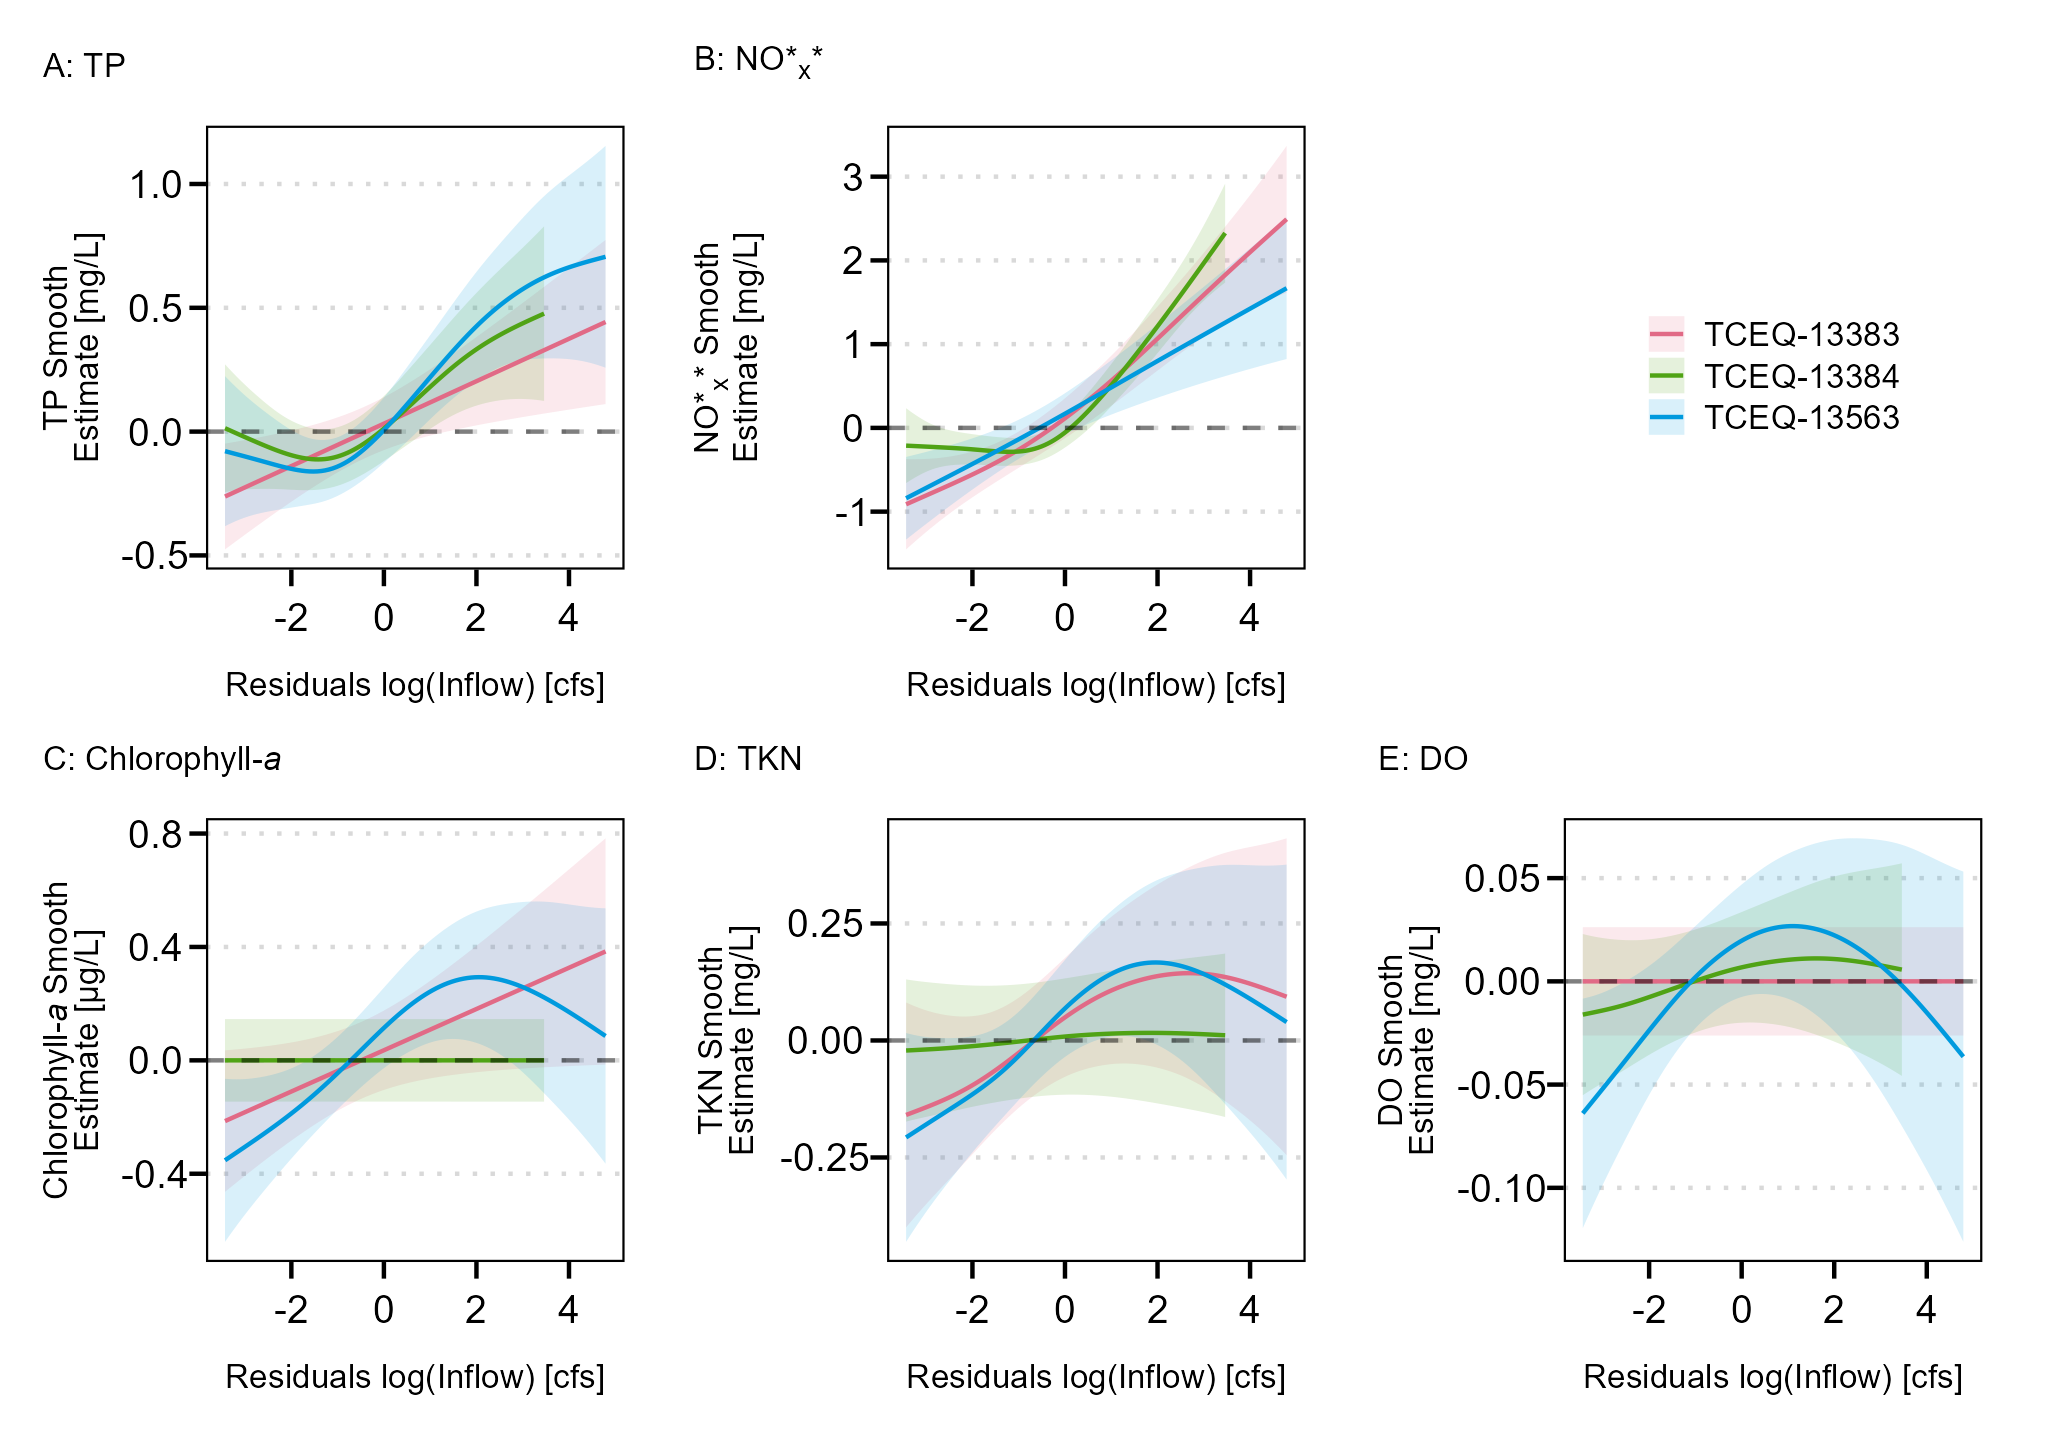
\includegraphics[width=1\linewidth,]{Schramm-2023-05-AS_files/figure-latex/fig6-1} 

}

\caption{Estimated effects of mean daily inflow residuals on mean TP, NO~*x*~, chlorophyll-*a*, TKN, and DO concentrations in Lavaca Bay obtained from flow estuary GAMs.}\label{fig:fig6}
\end{figure}

Increased TP loads resulted in nearly linear increases of TP
concentration at the upper- and mid-bay sites, TCEQ-13563 and TCEQ-13383
respectively (Figure~\ref{fig:fig7}). The relative effect size appeared
to much smaller than the effect of freshwater inflow alone. Increased
NO\textsubscript{3} loads only showed an effect at the lower-bay
TCEQ-13384 site. The effect was quite small compared to streamflow and
provided only small improvements to the model (\citet{tbl-table4}). As
noted above, nutrient loadings did not provide any explanation in
changes in the remaining assessed water quality parameters.

\begin{figure}

{\centering 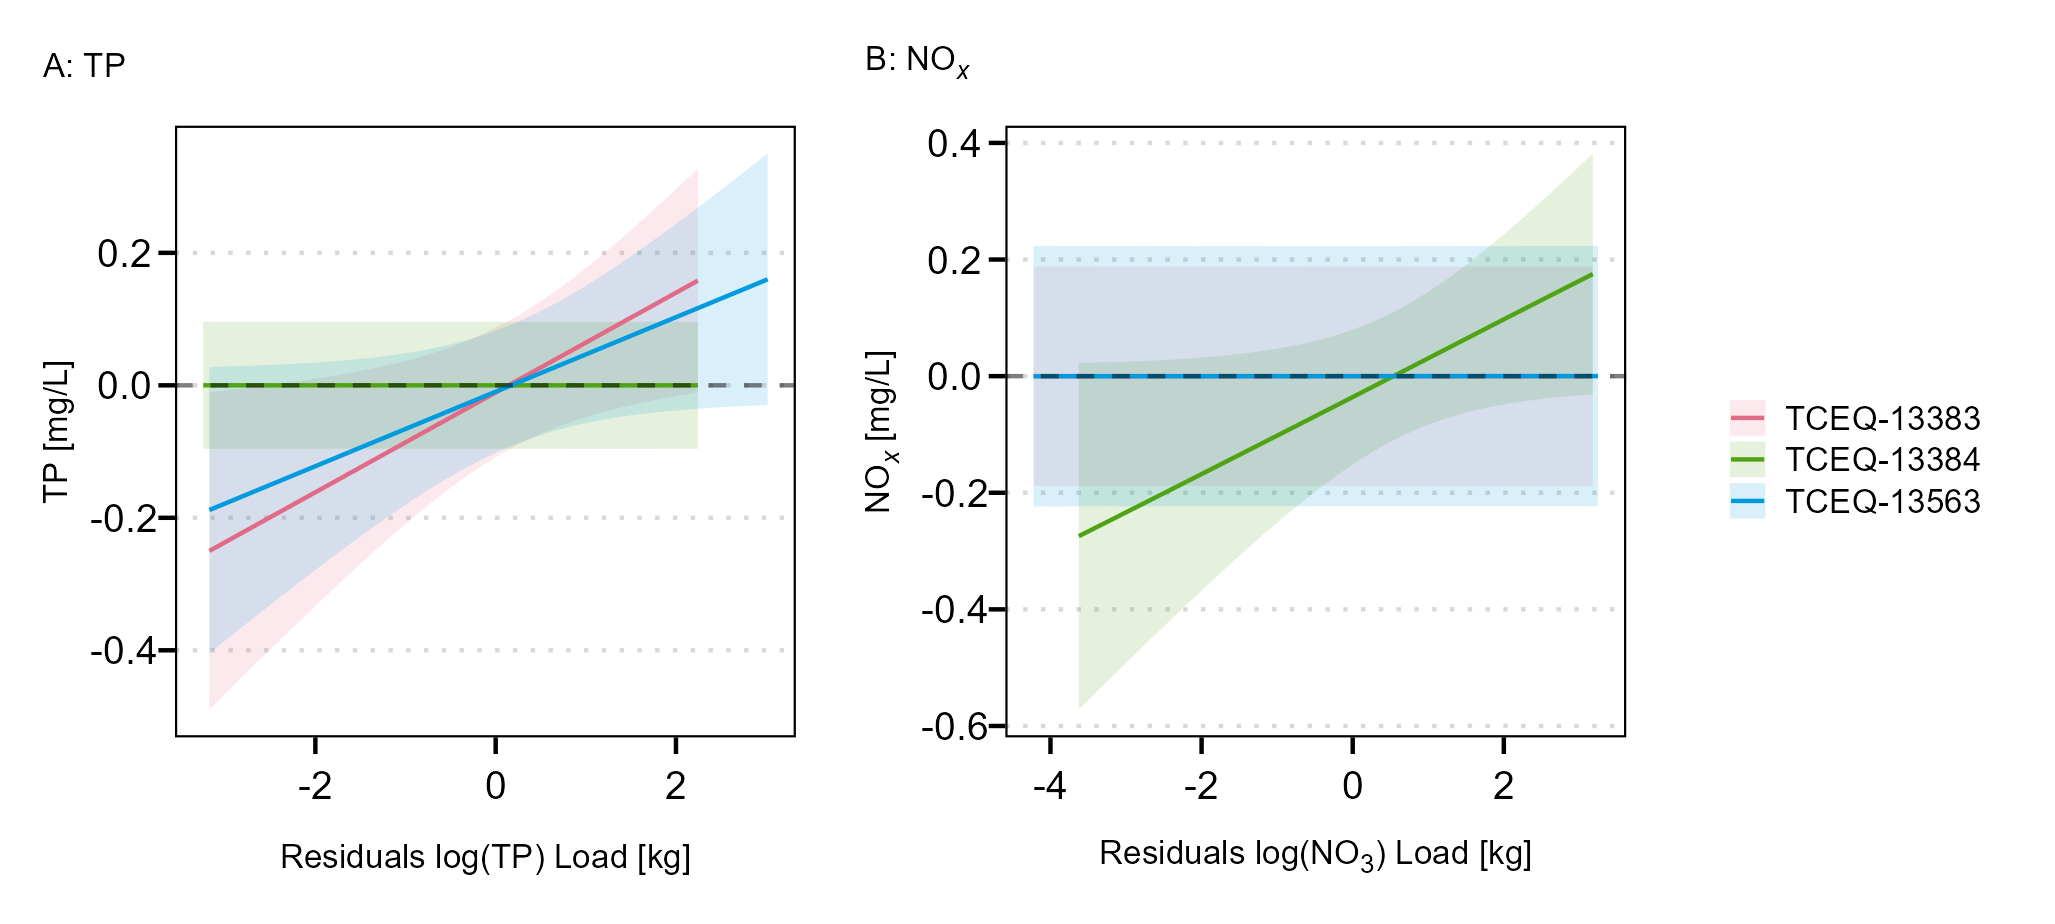
\includegraphics[width=1\linewidth,]{Schramm-2023-05-AS_files/figure-latex/fig7-1} 

}

\caption{Estimated effects of nutrient load residuals on TP and NO~*x*~ concentrations in Lavaca Bay obtained from flow+load estuary GAMs.}\label{fig:fig7}
\end{figure}

\hypertarget{discussion}{%
\section{Discussion}\label{discussion}}

\textbf{resume here}

TP and NO\textsubscript{3} loadings from the Lavaca Bay watershed showed
high inter-annual variability tied with changes in discharge. There is
little evidence for changes in flow-normalized TP loads in either
rivers. There is some evidence of recent decreases in flow-normalized
NO\textsubscript{3} loads in the Lavaca River. Although there is no work
directly correlating water quality planning and implementation efforts
in the watershed to water quality outcomes, efforts to increase
agricultural producer participation in the watershed have been ongoing
since 2016
\citep{schrammLavacaRiverWatershed2018, bertholdDirectMailingEducation2021}.
The decrease in flow-normalized NO\textsubscript{3} loads could be a
reflection of those collective efforts but further data collection and
research is required to support that statement.

Converted to average annual yield, the estimates of annual TP loads for
the Lavaca River are within the ranges in previous published studies
(\citet{tbl-table5};
\citep{dunnTrendsNutrientInflows1996, rebichSourcesDeliveryNutrients2011, omaniEstimationSedimentNutrient2014, wise_spatially_2019}).
It isn't obvious why TP estimates in
\citet{dunnTrendsNutrientInflows1996} were notably lower. Given that
none of the studies identify substantially sized trends in TP, it is is
possible that the period used in \citet{dunnTrendsNutrientInflows1996}
was drier on average than the other studies. The SPARROW models used in
\citet{rebichSourcesDeliveryNutrients2011} and
\citet{wise_spatially_2019} utilize a version of LOADEST in the
underlying load estimation procedure, so a difference due to methodology
alone is unlikely.

\begin{table}

\caption{\label{tab:table5}Comparisons of previously published estimates of mean annual TP yield at the Lavaca River site.}
\centering
\begin{tabular}[t]{llll}
\toprule
Reported Yield (kg$\cdot$km\textsuperscript{2}$\cdot$year\textsuperscript{-1}) & Approach & Time Period & Reference\\
\midrule
35.2 (28.8, 43.3)\textsuperscript{a} & GAM & 2005-2020 & This work\\
45.2 & SPARROW & 2000-2014 & \cite{wise_spatially_2019}\\
42 & SWAT & 1977-2005 & \cite{omaniEstimationSedimentNutrient2014}\\
20.81-91.58\textsuperscript{b} & SPARROW & 1980-2002 & \cite{rebichSourcesDeliveryNutrients2011}\\
28.9 & LOADEST & 1972-1993 & \cite{dunnTrendsNutrientInflows1996}\\
\bottomrule
\multicolumn{4}{l}{\rule{0pt}{1em}\textsuperscript{a} Mean of the annual point estimates and the lower and upper 95\% credible intervals.}\\
\multicolumn{4}{l}{\rule{0pt}{1em}\textsuperscript{b} Represents a binned value range from a choropleth map.}\\
\end{tabular}
\end{table}

Cross-validation of the GAM loading models indicated that GAMs performed
well on average at predicting daily nutrient loading values. The
variance in scores was very high indicating subsets of values were
problematic at characterizing functional relationships between nutrients
and predictors. Because all of the water quality data for these two
locations in the TCEQ databases were ambient water quality data,
collected to be representative of typical flow conditions, there were
few data at the highest portions of the flow-duration curve. It was
beyond the scope of the current study to evaluate the subsets of
cross-validation data and scores. However, the cross-validation
procedure is indicative that more robust sampling would be beneficial
for reducing prediction variance. Supplementary flow-biased monitoring
targeting storm- or high-flow conditions is recommended here to improve
the precision of GAM predictions
\citep{horowitzEvaluationSedimentRating2003, snelderEstimationCatchmentNutrient2017}.

The non-linear temporal water quality trends identified using GAMs
differed slightly from previously identified trends
\citep{bugica_water_2020}. This is not unexpected due to the different
time periods, different methodology, and generally small slopes
identified for most of the significant water quality parameters in prior
work. The trend in DO and cholorophyll-\emph{a} concentrations are
stable in comparison to other Texas estuaries that are facing larger
demands for freshwater diversions, higher population growth, and more
intense agricultural production
\citep{wetzWaterQualityDynamics2016, bugica_water_2020}. The trend of
increasing NO\textsubscript{\emph{x}} concentration at the upper-bay
TCEQ-13563 site and recent increases in TKN concentration at the mid-bay
TCEQ-13383 site are concerning due to the nitrogen limitation identified
in many Texas estuaries
\citep{gardnerNitrogenFixationDissimilatory2006, houTransformationFateNitrate2012, doradoUnderstandingInteractionsFreshwater2015, paudelRelationshipSuspendedSolids2019, wetz_exceptionally_2017}
and the relatively low ambient concentrations observed in Lavaca Bay.

The strong positive effect of freshwater inflow on
NO\textsubscript{\emph{x}}, TKN, and TP are suggestive of nonpoint
watershed sources, consistent with watershed uses and with other studies
relating freshwater inflow with nutrient concentrations in Lavaca Bay
and other estuaries
\citep{russell_effect_2006, caffreyHighNutrientPulses2007, peierlsNonmonotonicResponsesPhytoplankton2012, palmerImpactsDroughtsLow2015, ciraPhytoplanktonDynamicsLowinflow2021}.
Inflow had a non-linear relationship with TKN at the two upstream sites,
with TKN increasing as freshwater inflow transitioned from low to
moderate levels. At higher freshwater inflows, the effect was
attenuated, possibly indicating a flushing effect at higher freshwater
inflow. No relationship between TKN and freshwater inflow were observed
at TCEQ-13384 located in the lower reach of Lavaca Bay. Tidal flushing
from Matagorda Bay could be responsible for diluting TKN and acting as a
control on the effects of freshwater inflow in lower reaches of Lavaca
Bay. Previous work suggests the processing of organic loads in the upper
portions of Lavaca Bay might reduce the transport of nutrients into the
lower reaches of the Bay \citep{russell_effect_2006}.

Freshwater inflow had a strong positive effect on chlorophyll-\emph{a}
at the upper- and mid-bay sites. The upper-bay site, TCEQ-13563, showed
decreases in chlorophyll-\emph{a} at the highest freshwater inflow
volumes. Freshwater flushing or increases in turbidity are associated
with decreases in chlorophyll-\emph{a} in other estuaries
\citep{peierlsNonmonotonicResponsesPhytoplankton2012, cloernPhytoplanktonPrimaryProduction2014}.
No relationships between inorganic nitrogen or TP loadings with
chlorophyll-\emph{a} were observed. Due to the lack of TKN loading
information, no assessment between organic nitrogen loads and
chlorophyll-\emph{a} were possible.

Although other studies have identified complex relationships between
estuary nutrient concentrations, nutrient loading and
chlorophyll-\emph{a} concentrations in Texas estuaries
\citep{ornolfsdottirNutrientPulsingRegulator2004, doradoUnderstandingInteractionsFreshwater2015, ciraPhytoplanktonDynamicsLowinflow2021, tominackVariabilityPhytoplanktonBiomass2022},
this study specifically used flow-adjusted freshwater derived nutrient
loads to parse out contributions from changes in nutrient loadings while
accounting for variations in load due to flow. Loading GAMs indicated no
evidence of changes in flow-normalized TP loads in either river, and no
changes in flow-normalized NO\textsubscript{3} loads in the Navidad
River. The small changes in flow-normalized NO\textsubscript{3} loads in
the Lavaca River are probably masked under most conditions by discharge
from the Navidad River. Given the relatively small variation in
flow-normalized loads, it can be expected that they would contribute
little to the variance in downstream water quality.

GAMs did not identify responses in DO concentration to inflows or
nutrient loads. The seasonality term in the temporal GAM models
explained a substantial amount of DO variation at all of the sites.
Responses of estuary metabolic processes and resulting DO concentrations
can be quite complicated and often locally specific
\citep{caffreyFactorsControllingNet2004}. While the lack of total
nitrogen or TKN loading data hinders interpretation, the large seasonal
effect on DO suggests physical factors play an important role and should
be included in future models. Prior work suggests that Lavaca Bay may
not be limited by nutrients alone, with high turbidity or nutrient
processing in upper portions of the Bay or intertidal river limiting
production \citep{russell_effect_2006}. Finally, it is reasonable to
assume that fluctuations in DO may not occur immediately in response to
nutrient pulses or freshwater inflow. Work has has shown that various
water quality parameters may have lagged effects lasting days or even
months following storms and large discharge events
\citep{mooneyWatershedExportEvents2012a, wetzExtremeFutureEstuaries2013, bukaveckasInfluenceStormEvents2020, walkerTimescalesMagnitudeWater2021}.
However, our work only evaluates responses to loading and inflows
occuring the day of water quality observations.

\hypertarget{conclusion}{%
\section{Conclusion}\label{conclusion}}

GAM models appear to provide reliable estimates of nutrient loads in the
Lavaca Bay watershed. However, additional flow-biased data collection
efforts would decrease the prediction variance and improve accuracy at
critical high flow events. Ongoing projects will fill data gaps for
total nitrogen and TKN loading. This study, consistent with others along
the Texas coast, found strong effects of freshwater flow on nutrient and
chlorophyll-\emph{a} concentrations. DO concentrations, dominated by
seasonal effects, did not show strong direct responses to freshwater
flow. Small variance in flow-adjusted nutrient loads indicates that (1)
there have been limited changes in non-point sources of nutrients and
(2) that there isn't strong evidence that those small changes have had
effects on chlorophyll-\emph{a} or dissolved oxygen in Lavaca Bay.
Although the study did not identify strong responses to changes in
nutrient loading, this does provide a baseline assessment for future
water quality management activities in the watershed.

\backmatter

\bmhead{Acknowledgments}

The author extends thanks to Dr.~Mike Wetz (Harte Research Institute,
Texas A\&M Corpus Christi), Chad Kinsfather and Partick Brzozowski
(Lavaca-Navidad River Authority), Brian Koch (Texas State Soil and Water
Conservation Board), Bill Balboa (Matagorda Bay Foundation), Jason
Pinchbeck (Texas General Land Office) and the Lavaca Bay Foundation for
supporting development of this project and providing valuable feedback.

\hypertarget{declarations}{%
\section*{Declarations}\label{declarations}}
\addcontentsline{toc}{section}{Declarations}

\bmhead{Funding}

This project was funded in part by a Texas Coastal Management Program
grant approved by the Texas Land Commissioner, providing financial
assistance under the Coastal Zone Management Act of 1972, as amended,
awarded by the National Oceanic and Atmospheric Administration (NOAA),
Office for Coastal Management, pursuant to NOAA Award
No.~NA21NOS4190136. The views expressed herein are those of the
author(s) and do not necessarily reflect the views of NOAA, the U.S.
Department of Commerce, or any of their subagencies.

\bmhead{Data Availability}

Reproducible code and datasets generated during this study are available
in the Zenodo repository, \url{https://doi.org/10.5281/zenodo.733075}.

\bibliography{bibliography.bib}


\end{document}
